\documentclass[12pt, a4paper]{report}

% --- Core Typography & Encoding Packages ---
\usepackage[utf8]{inputenc}
\usepackage[T1]{fontenc}
\usepackage[english]{babel}
\usepackage{graphicx} 
\usepackage{geometry} 
\usepackage{titlesec} 
\usepackage{setspace} 
\usepackage{multirow}
\usepackage{amsmath} 
\usepackage{algorithm}
\usepackage{algorithmic}
\usepackage{longtable}
\usepackage{booktabs}
\usepackage{array}
\usepackage{newtxtext,newtxmath}
\usepackage{microtype}
\usepackage{caption}
\usepackage{subcaption}

% --- Hyperlink & Document Geometry Configuration ---
\geometry{
    top=2.5cm,
    bottom=2.5cm,
    left=3.0cm, 
    right=2.5cm
}
\setstretch{1.5} 

\usepackage[
    pdftex,
    colorlinks=true,
    linkcolor=black,
    citecolor=black,
    urlcolor=blue,
    bookmarks=true,
    bookmarksnumbered=true,
    pdfstartview={FitH}
]{hyperref}

% Remove chapter numbers from title format to match faculty template style
\titleformat{\chapter}[display]
  {\normalfont\huge\bfseries}{\chaptertitlename\ \thechapter}{20pt}{\Huge}

\begin{document}

% ==========================================
%               TITLE PAGE
% ==========================================
\begin{titlepage}
\begin{center}
{\Large{\textsc{Sri Lanka Institute of Information Technology}}} \\
\vspace{2mm}
\rule[0.1cm]{15.8cm}{0.1mm} \\
\vspace{-5mm}
\rule[0.5cm]{15.8cm}{0.6mm} \\
\vspace{1.5cm}

{\LARGE \textbf{PROTECTIVA: A MULTI-MODAL EDGE-AI FRAMEWORK FOR PEDIATRIC RESIDENTIAL SAFETY}} \\
\vspace{1.2cm}

{\Large \textbf{INDIVIDUAL RESEARCH THESIS}} \\
\vspace{1cm}

{\large \textbf{K. Vidusha Upashalya De Abrew}} \\
{\large (IT22168054)} \\
\vspace{1cm}

{\large \textbf{Individual Component: Audio Guardian and Frontend Orchestration}} \\
{\large Group Identifier: RP\_WE\_G104} \\
\vspace{1.5cm}

{\large Report submitted in partial fulfilment of the requirements for the degree of} \\
{\large \textbf{Bachelor of Science (Honours) in Information Technology}} \\
{\large Specializing in Software Engineering} \\
\vspace{1.5cm}

{\large Department of Information Technology} \\
{\large Faculty of Computing} \\
{\large Sri Lanka Institute of Information Technology} \\
{\large Sri Lanka} \\
\vfill
{\large \today}
\end{center}
\end{titlepage}

% ==========================================
%               DECLARATION
% ==========================================
\pagenumbering{roman}
\setcounter{page}{2}

\chapter*{DECLARATION AND SUPERVISOR CERTIFICATION}
\addcontentsline{toc}{chapter}{DECLARATION AND SUPERVISOR CERTIFICATION}

\textbf{Candidate Declaration.} I declare that this thesis is my own work and does not incorporate, without acknowledgement, material previously submitted for a degree or diploma at any university or institute of higher learning. To the best of my knowledge and belief, it contains no material previously published or written by another person except where due acknowledgement is made in the text. I grant the Sri Lanka Institute of Information Technology the non-exclusive right to reproduce and distribute this thesis, in whole or in part, in print, electronic, or other media, while retaining the right to use the content in future work.
\vspace{0.6cm}

\noindent Student Name: K. Vidusha Upashalya De Abrew \\
Student ID: IT22168054 \\
Signature: \hrulefill \hspace{1cm} Date: \hrulefill
\vspace{1.0cm}

\noindent \textbf{Academic Integrity and Generative AI Disclosure.} In full compliance with SLIIT academic integrity regulations and institutional generative artificial intelligence policies, I declare that generative AI tools utilized during this research project were confined exclusively to code scaffolding, LaTeX syntax remediation, and grammatical styling assistance. All theoretical models, algorithmic formulations, acoustic data processing pipelines, experimental evaluations, and analytical conclusions presented herein represent the authentic and verified work of the author, as detailed in Appendix~B.
\vspace{1.0cm}

\noindent \textbf{Supervisor Certification.} The above candidate has carried out this research project for the bachelor's degree individual thesis under my direct supervision.
\vspace{0.6cm}

\begin{table}[htbp]
\centering
\begin{tabular}{@{} p{0.48\linewidth} p{0.28\linewidth} p{0.18\linewidth} @{}}
\toprule
\textbf{Role and Name} & \textbf{Signature} & \textbf{Date} \\
\midrule
Supervisor: Prof. Pradeep Abeygunawardhana & \hrulefill & \hrulefill \\
\bottomrule
\end{tabular}
\end{table}

\clearpage

% ==========================================
%               ABSTRACT & ACKNOWLEDGEMENTS
% ==========================================
\chapter*{ABSTRACT}
\addcontentsline{toc}{chapter}{ABSTRACT}
Single-sensor domestic child-safety monitors suffer from severe acoustic blind spots, catastrophic intensity bias, and high false-positive notification rates that induce caregiver alert fatigue. This thesis details the design, algorithmic formulation, firmware implementation, and empirical validation of the \textbf{Audio Guardian} subsystem---a privacy-preserving, edge-native acoustic monitoring and biometric verification component within the multi-modal Protectiva framework. Operating under a strict ``Zero-Raw-Audio'' transmission doctrine, the edge sensing node captures continuous ambient audio via an INMP441 digital MEMS microphone interfaced to an Espressif ESP32-S3 microcontroller (\$15~USD BOM). The edge node executes hardware-accelerated Digital Signal Processing (DSP) to compute a 120-channel multi-spectral dynamic tensor (40 base MFCCs + 40 first-order $\Delta$ velocity + 40 second-order $\Delta\Delta$ acceleration coefficients across 150 temporal frames) while immediately zero-overwriting and purging raw volatile pulse-code modulation (PCM) waveforms via DMA buffers. 

Classification is performed by \textbf{AudioThreatNet}, a hybrid 1D-CNN+LSTM neural architecture (97,602 parameters, 14.27~MFLOPs) specifically engineered to model the rapid non-linear onset, subharmonic bifurcations, and acoustic roughness characteristic of pediatric distress screams. To prevent alert fatigue caused by benign, high-decibel household speech, a deterministic second-stage biometric verification gate extracts a 64-dimensional vocal tract formant embedding and calculates Cosine Distance against enrolled parental voice profiles, instantaneously overriding false alarms without suppressing unattended child distress. Benchmarked against a stratified held-out evaluation corpus derived from the RAVDESS and ESC-50 datasets, AudioThreatNet achieves an overall classification accuracy of \textbf{98.0\%}, a safety-critical threat recall of \textbf{96.0\%}, a threat precision of \textbf{100.0\%}, a specificity of \textbf{100.0\%}, and an area under the ROC curve (ROC-AUC) of \textbf{0.9976} (PR-AUC = \textbf{0.9977}). A 2,000-iteration non-parametric bootstrap analysis confirms a 95\% confidence interval of [90.0\%, 100.0\%] for threat recall, while Wilson Score and Clopper-Pearson exact intervals formally bound the false alarm rate within [0.0\%, 7.13\%]. End-to-end telemetry latency across the edge-cloud-mobile pipeline measures \textbf{195.4\,ms}, comfortably satisfying the sub-200\,ms real-time life-safety constraint. \\

\noindent \textbf{Keywords:} Edge AI, Acoustic Threat Detection, 1D-CNN+LSTM, Vocal Tract Biometrics, Cosine Distance, Child Safety, ESP32-S3, Alert Fatigue.

\clearpage

\chapter*{ACKNOWLEDGEMENTS}
\addcontentsline{toc}{chapter}{ACKNOWLEDGEMENTS}
I express my deepest gratitude and sincere appreciation to my research supervisor, Prof. Pradeep Abeygunawardhana, for his intellectual leadership, invaluable mentorship, and continuous encouragement throughout the inception, design, and execution of this thesis. His rigorous academic standards and constructive critiques were instrumental in shaping the methodology and scientific depth of this research.

I extend my appreciation to the academic and administrative staff of the Department of Information Technology and the Faculty of Computing at the Sri Lanka Institute of Information Technology (SLIIT) for providing the high-performance computing facilities and supportive academic environment essential for completing this engineering endeavour.

Finally, I dedicate my heartfelt gratitude to my family and colleagues for their enduring patience, understanding, and unwavering moral support throughout this demanding academic journey.

\clearpage

% ==========================================
%               LISTS
% ==========================================
\tableofcontents
\listoffigures
\listoftables

\clearpage

\chapter*{LIST OF ABBREVIATIONS}
\addcontentsline{toc}{chapter}{LIST OF ABBREVIATIONS}
\begin{longtable}{@{} p{0.22\linewidth} p{0.73\linewidth} @{}}
\toprule
\textbf{Abbreviation} & \textbf{Definition} \\
\midrule
\endhead
AED & Acoustic Event Detection \\
ANN & Artificial Neural Network \\
AOP & Acoustic Overload Point \\
API & Application Programming Interface \\
AUC & Area Under the Curve \\
BOM & Bill of Materials \\
CDC & Change Data Capture \\
CNN & Convolutional Neural Network \\
CRNN & Convolutional Recurrent Neural Network \\
DFT & Discrete Fourier Transform \\
DMA & Direct Memory Access \\
DSP & Digital Signal Processing \\
DTW & Dynamic Time Warping \\
EAS & Expo Application Services \\
ESC & Environmental Sound Classification \\
FAR & False Alarm Rate \\
FFT & Fast Fourier Transform \\
FLOPs & Floating-Point Operations \\
FPR & False Positive Rate \\
GDPR & General Data Protection Regulation \\
HaaS & Hardware-as-a-Service \\
HPSS & Harmonic-Percussive Source Separation \\
I2S & Inter-IC Sound \\
ICC & Infant Cry Classification \\
IoT & Internet of Things \\
LSTM & Long Short-Term Memory \\
MACs & Multiply-Accumulate Operations \\
MCU & Microcontroller Unit \\
MEMS & Micro-Electro-Mechanical Systems \\
MFCC & Mel-Frequency Cepstral Coefficients \\
MLP & Multi-Layer Perceptron \\
NLOS & Non-Line-of-Sight \\
PCM & Pulse-Code Modulation \\
PR & Precision-Recall \\
RAG & Retrieval-Augmented Generation \\
RAVDESS & Ryerson Audio-Visual Database of Emotional Speech and Song \\
RMS & Root-Mean-Square \\
ROC & Receiver Operating Characteristic \\
SaaS & Software-as-a-Service \\
SER & Speech Emotion Recognition \\
SPL & Sound Pressure Level \\
SRAM & Static Random-Access Memory \\
SVM & Support Vector Machine \\
TLS & Transport Layer Security \\
TPR & True Positive Rate \\
ULP & Ultra-Low-Power \\
VAD & Voice Activity Detection \\
WLAN & Wireless Local Area Network \\
ZCR & Zero-Crossing Rate \\
\bottomrule
\end{longtable}

\clearpage

% ==========================================
%               MAINMATTER
% ==========================================
\pagenumbering{arabic}
\setcounter{page}{1}

\chapter{INTRODUCTION}

\section{Overall Project Context}
Child physical safety within residential and domestic environments represents an enduring public health challenge and societal concern. Epidemiological analyses confirm that young children, particularly those transitioning through early developmental stages between 4 and 8 years of age, exhibit increasing physical mobility and domestic exploration while lacking the cognitive risk-awareness required to anticipate environmental hazards. Unintentional domestic injuries, falls, acute physical distress, and unsupervised domestic conflicts represent leading causes of pediatric morbidity worldwide.

Historically, domestic safety monitoring has relied heavily on single-modality surveillance paradigms, most prominently closed-circuit television (CCTV) cameras, commercial baby monitors, or simple smart-home audio sensors. However, these conventional solutions suffer from critical architectural deficiencies:
\begin{enumerate}
    \item \textbf{Visual Occlusion and Spatial Blind Spots:} Optical cameras require uncompromised direct line-of-sight (LOS). Domestic interiors contain architectural partitions, walls, furniture, and closed doors that create pervasive surveillance blind spots where physical trauma frequently occurs.
    \item \textbf{Intrusive Privacy Violations:} Continuous streaming of high-definition video and raw acoustic waveforms across third-party cloud infrastructure creates severe domestic privacy hazards, conflicting with international data protection mandates.
    \item \textbf{Acoustic Intensity Bias and Caregiver Alert Fatigue:} Traditional nursery monitors rely exclusively on scalar amplitude thresholds. Consequently, benign high-decibel household transients (e.g., dropped kitchenware, blender activation, television action scenes) trigger persistent false alarms, rapidly desensitizing parents and inducing caregiver alert fatigue.
\end{enumerate}

To comprehensively address these systemic vulnerabilities, the \textbf{Protectiva} framework was conceptualized as an integrated, multi-modal edge-AI surveillance and legal decision-support platform tailored for children aged 4 to 8 years. As illustrated in the systemic taxonomy, Protectiva incorporates four complementary sub-systems:
\begin{itemize}
    \item \textbf{Vision Guardian:} Edge-based computer vision utilizing lightweight convolutional neural networks for human pose estimation and hazardous proximity tracking.
    \item \textbf{Audio Guardian:} A privacy-preserving, edge-native bio-acoustic monitoring and vocal biometric verification subsystem (the subject of this thesis).
    \item \textbf{Legal RAG System:} A specialized Retrieval-Augmented Generation regulatory advisory pipeline providing jurisdictional context for child welfare incidents.
    \item \textbf{Data Fusion Dashboard:} A synchronized mobile and web presentation layer orchestrating telemetry, presence state estimation, and emergency escalation.
\end{itemize}

\section{Individual Component Context: The Audio Guardian}
Within the Protectiva ecosystem, the author was solely responsible for the conception, theoretical derivation, embedded firmware engineering, deep learning pipeline, and mobile orchestration of the \textbf{Audio Guardian}. 

Bio-acoustic surveillance provides an essential complementary modality to optical tracking. Sound propagation is omnidirectional and inherently non-line-of-sight (NLOS), capable of diffracting around household obstructions and penetrating acoustic pathways across occluded domestic spaces where optical cameras are strictly prohibited due to privacy constraints (e.g., bathrooms and private bedrooms). The Audio Guardian bridges the gap between low-cost physical edge sensing and cloud intelligence by pairing an ultra-low-cost Espressif ESP32-S3 microcontroller and an INMP441 MEMS digital microphone with a high-throughput FastAPI inference server and a React Native mobile supervisory application.

\section{Problem Statement}
Commercial acoustic nursery monitors and smart home surveillance apparatuses exhibit two interrelated, systemic failures: \textit{Intensity Bias} and \textit{Caregiver Alert Fatigue}. 

Current market monitors rely overwhelmingly on trivial scalar sound pressure level (SPL) or Root-Mean-Square (RMS) amplitude thresholding. These devices trigger notifications whenever the ambient energy in an acoustic window exceeds a preset decibel ceiling (e.g., 75--80~dB). In an active domestic household, benign events such as loud vacuum cleaners, exuberant laughter, high-volume television dialogue, or an adult parent shouting across a hallway easily reach 80--90~dB SPL. Because scalar monitors lack semantic signal intelligence, they classify every high-amplitude sound as an emergency, generating frequent false-positive alerts. In clinical and domestic human factors engineering, persistent false alarms trigger \textit{Caregiver Alert Fatigue} \cite{ref_sendelbach2013}, driving caregivers to mute, ignore, or completely disconnect safety monitors, with potentially catastrophic consequences when genuine pediatric distress occurs.

\section{Research Gap}
A rigorous analysis of contemporary academic literature and commercial products reveals an unresolved dichotomy in acoustic domestic surveillance:
\begin{enumerate}
    \item \textbf{Heuristic, Low-Intelligence Edge Appliances:} Embedded commercial monitors operate purely on basic time-domain energy metrics to fit within constrained microcontroller memory. They exhibit poor selectivity, generating unmanageable false alarms.
    \item \textbf{Centralized, Privacy-Violating Cloud Architectures:} Modern deep-learning acoustic classifiers operate on high-parameter architectures that stream continuous, uncompressed pulse-code modulation (PCM) audio to remote corporate clouds. This creates severe wiretapping and interception risks, directly violating privacy-by-design standards.
\end{enumerate}
No reported system successfully integrates lightweight, real-time edge multi-spectral parameterization with on-chip raw waveform purging, deep sequence classification of acute pediatric distress, and deterministic biometric false-alarm suppression under an accessible bill-of-materials constraint ($<\$\$20$~USD).

\section{Aim and Objectives}
The overarching aim of this research is to design, implement, and empirically validate the \textbf{Audio Guardian}: an edge-native, privacy-preserving bio-acoustic monitoring framework that accurately detects acute pediatric distress screams while deterministically eliminating false alarms caused by benign domestic sounds and caregiver vocalizations.

Specific technical objectives include:
\begin{itemize}
    \item \textbf{Objective 1:} Formulate and deploy an embedded digital signal processing (DSP) pipeline on the ESP32-S3 to compute a 120-channel multi-spectral feature tensor (MFCC + $\Delta$ + $\Delta\Delta$) within on-chip SRAM, enforcing immediate volatile zero-overwriting purge of raw PCM audio.
    \item \textbf{Objective 2:} Design, train, and benchmark a hybrid 1D-CNN+LSTM neural network (\textbf{AudioThreatNet}) optimized to discriminate acute pediatric pain screams from benign household transients.
    \item \textbf{Objective 3:} Engineer a text-independent biometric speaker verification module based on 64-dimensional vocal tract formant embeddings and Cosine Distance gating to verify authorized caregivers and eliminate false alarms.
    \item \textbf{Objective 4:} Construct an enterprise-grade mobile orchestration frontend in React Native featuring a 3-step guided voice enrollment wizard and sub-200\,ms dual-backend failover resilience.
    \item \textbf{Objective 5:} Execute rigorous empirical benchmarking, statistical bootstrapping, exact binomial bounding, and ablation studies against standard acoustic corpora.
\end{itemize}

\section{Research Questions}
This investigation is guided by three core research questions:
\begin{itemize}
    \item \textbf{RQ1:} Can an ultra-low-cost (\$15~USD) microcontroller (ESP32-S3) execute continuous 120-channel multi-spectral feature extraction within constrained internal memory limits (512~KB SRAM) while maintaining real-time processing throughput?
    \item \textbf{RQ2:} To what degree does cascading 1D temporal convolutions with recurrent LSTM sequence modeling improve acute distress classification accuracy and recall over standard multi-layer perceptrons, 1D-CNNs, and dense 2D-CNN baselines?
    \item \textbf{RQ3:} Can a secondary 64-dimensional vocal tract biometric gate reliably suppress benign caregiver vocal transients to achieve a zero false alarm rate ($0.0\%$ FAR) without degrading safety-critical threat recall?
\end{itemize}

\section{Scope, Limitations, and Assumptions}
The operational scope of the Audio Guardian is established for pediatric safety monitoring of children aged 4 to 8 years within residential domestic interiors. The edge physical node is constrained to the Espressif ESP32-S3-WROOM-1 microcontroller interfaced via I2S to an INMP441 omnidirectional MEMS digital microphone. Acoustic events exceeding the microphone's physical 120~dB Acoustic Overload Point (AOP) will undergo hardware-level clipping. Continuous operation assumes standard residential mains power with a local 2.4~GHz Wi-Fi (802.11b/g/n) network.

\section{Individual Contribution}
The author was exclusively responsible for:
\begin{enumerate}
    \item Deriving the acoustic bio-mechanics and mathematical parameterization of the 120-channel dynamic tensor pipeline.
    \item Authoring the ESP32-S3 embedded C++/Arduino firmware implementing DMA double-buffering, FFT framing, and the volatile memory zero-overwriting purge routine.
    \item Designing, training, optimizing, and evaluating the AudioThreatNet deep neural architecture in PyTorch.
    \item Formulating and validating the 64-dimensional text-independent vocal tract biometric embedding and Cosine Distance decision gate.
    \item Engineering the FastAPI backend microservice and the cross-platform React Native supervisory application, including the 3-Step Biometric Voice Enrollment Wizard.
    \item Executing all empirical evaluations, statistical bootstrapping, exact binomial intervals, and ablation studies.
\end{enumerate}

\section{Thesis Structure}
The remainder of this thesis is structured as follows: Chapter~2 presents a systematic literature review covering pediatric acoustic biomechanics, TinyML constraints, and existing systems. Chapter~3 details the research methodology, framing parameters, and dataset partitioning. Chapter~4 outlines the system architecture and mathematical biometric formulation. Chapter~5 discusses implementation, testing, and API specifications. Chapter~6 presents empirical results, ROC/PR curves, and latency breakdowns. Chapter~7 provides a critical discussion and ablation analysis. Chapter~8 examines commercialisation, sustainability, and bandwidth optimization. Chapter~9 concludes the thesis and outlines future directions.

\chapter{LITERATURE REVIEW AND RELATED WORK}

\section{Review Method and Scope}
To establish a rigorous theoretical and empirical foundation for the Audio Guardian subsystem, a systematic literature review was executed following the guidelines of Kitchenham et al.~\cite{ref_kitchenham2007} and the PRISMA statement~\cite{ref_prisma2020}. The objective was to survey and synthesize peer-reviewed academic literature across five converging domains: Acoustic Event Detection (AED), Speech Emotion Recognition (SER), embedded TinyML digital signal processing, acoustic biomechanics of pediatric dysphonia, and biometric speaker verification.

The literature search queried primary electronic databases including IEEE Xplore, the ACM Digital Library, ScienceDirect (Elsevier), SpringerLink, PubMed, and DCASE challenge proceedings. Boolean search expressions combined standardized keywords: \texttt{("acoustic distress" OR "scream detection" OR "pediatric cry") AND ("TinyML" OR "embedded DSP" OR "edge AI") AND ("false alarm suppression" OR "speaker verification" OR "biometrics")}. Articles were screened based on methodological rigor, peer-reviewed status, relevance to domestic or clinical acoustic surveillance, and applicability to resource-constrained embedded hardware.

\section{Domain and Theoretical Foundations}

\subsection{Acoustic Bio-Mechanics of Pediatric Dysphonia and Deterministic Chaos}
Human speech production is classically modeled using the source-filter acoustic theory formulated by Fant~\cite{ref_fant1960} and extended by Titze~\cite{ref_titze2000}. Under modal phonation, steady pulmonic airflow induces self-sustained, quasi-periodic oscillations of the bilateral vocal folds within the larynx. This generates an acoustic glottal volume velocity wave characterized by a fundamental frequency ($F_0$) and integer-multiple harmonic overtones ($2F_0, 3F_0, \dots$). As this source wave traverses the supraglottal vocal tract, resonant frequencies known as formants ($F_1, F_2, F_3$) sculpt the timbral spectral envelope.

However, during genuine pediatric pain, terror, or acute physical injury, neuro-motor activation under extreme sympathetic autonomic arousal destabilizes this linear phonatory regime~\cite{ref_fitch2002}. Subglottal air pressure surges precipitously, frequently exceeding $25\text{--}40\text{ cm }\text{H}_2\text{O}$ (in contrast to normal conversational levels of $5\text{--}8\text{ cm }\text{H}_2\text{O}$). When coupled with intense, asymmetric hyperadduction of the laryngeal musculature, the mechanical restoring forces of the vocal folds become non-linear, triggering three distinct bio-acoustic phenomena:
\begin{enumerate}
    \item \textbf{Subharmonic Bifurcations and Period Doubling:} Non-linear coupling causes the vibrating vocal fold tissues to desynchronize. In accordance with non-linear dynamical systems theory~\cite{ref_wilden1998}, this bifurcation introduces fractional subharmonic spectral components ($\frac{F_0}{2}, \frac{F_0}{3}, \frac{3F_0}{2}$) that appear intercalated between standard glottal harmonics.
    \item \textbf{Biphonation:} Simultaneous, independent oscillations of the left and right vocal folds at differing fundamental rates ($F_0$ and $F_{0}'$) create pronounced frequency beating and complex sidebands.
    \item \textbf{Deterministic Chaos and Acoustic Roughness:} Severe physical distress drives the laryngeal tissue into chaotic oscillation, completely destroying harmonic periodicity and generating a broad, turbulent acoustic spectrum. As demonstrated by Arnal et al.~\cite{ref_arnal2015}, human screams occupy a privileged acoustic niche characterized by temporal modulation rates between 30 and 150~Hz, termed \textit{acoustic roughness}. Psychophysically, this roughness selectively triggers the basolateral amygdala in human listeners, provoking immediate fear responses.
    \item \textbf{Pediatric Formant Shifts:} In children aged 4 to 8 years, the shortened vocal tract length ($\approx 10\text{--}12\text{ cm}$) raises the baseline conversational pitch to 250--350~Hz. Under acute distress, fundamental frequencies spike violently into the 800--1500~Hz band, accompanied by severe formant clustering in the 2.5~kHz to 5.0~kHz distress band~\cite{ref_sheinkopf2012, ref_mccofie2026}.
\end{enumerate}

\subsection{Digital Signal Processing and Multi-Spectral Parameterization}
Because raw acoustic pressure waves are non-stationary, embedded digital signal processing must transform discrete time-domain samples into compact, discriminative time-frequency representations~\cite{ref_oppenheim2010}. The Mel-Frequency Cepstral Coefficients (MFCCs) pioneered by Davis and Mermelstein~\cite{ref_davis1980} parameterize the spectral envelope along a non-linear, perceptually motivated Mel scale that mirrors the human cochlea:
\begin{equation}
m = 2595 \log_{10}\left(1 + \frac{f}{700}\right)
\end{equation}
As established by Rabiner and Juang~\cite{ref_rabiner1993} and Zhou et al.~\cite{ref_zhou2011}, static cepstral vectors capture stationary timbral identity but fail to represent the explosive velocity and acceleration trajectories of distress screams. To capture dynamic temporal transitions, static coefficients are augmented with first-order orthogonal regression polynomial derivatives ($\Delta$, velocity) and second-order acceleration ($\Delta\Delta$) coefficients:
\begin{equation}
d_t = \frac{\sum_{n=1}^{N} n (c_{t+n} - c_{t-n})}{2 \sum_{n=1}^{N} n^2}
\end{equation}
Stacking 40 base MFCCs, 40 $\Delta$, and 40 $\Delta\Delta$ coefficients produces a 120-channel multi-spectral dynamic tensor. Capturing these signals on physical edge hardware requires high-fidelity digital conversion. The InvenSense INMP441 omnidirectional MEMS microphone~\cite{ref_invensense2014} integrates a 24-bit $\Sigma\Delta$ analog-to-digital converter and an industry-standard Inter-IC Sound (I2S) serial bus, providing a 61~dBA signal-to-noise ratio and a 120~dB Acoustic Overload Point (AOP).

\subsection{TinyML Paradigms and Computational Intractability of Dense 2D-CNNs}
The deployment of deep machine learning models onto resource-constrained embedded microcontrollers is formalized under the TinyML paradigm~\cite{ref_almaini2025}. In recent acoustic event detection literature, researchers have frequently deployed two-dimensional Convolutional Neural Networks (2D-CNNs) trained on high-resolution Mel-spectrogram images ($128 \times 150$)~\cite{ref_hershey2017}. While 2D-CNNs achieve strong classification accuracy in cloud environments, they are computationally intractable for domestic edge microcontrollers.

A standard 3-block 2D-CNN operating on a $128 \times 150$ spectrogram requires over $105.4\text{ MFLOPs}$ per inference window. Furthermore, calculating intermediate activation tensors (e.g., $64\text{ channels} \times 64 \times 75 \times 4\text{ bytes} \approx 1.23\text{ MB}$) vastly exceeds the on-chip internal Static Random-Access Memory (SRAM) of microcontrollers such as the Espressif ESP32-S3 (512~KB total SRAM, with only $\approx 320\text{ KB}$ available as contiguous heap). While external Pseudo-SRAM (PSRAM) can be attached, accessing PSRAM over an external SPI bus introduces severe bus contention with active Wi-Fi Direct Memory Access (DMA), spiking inference latency to $> 300\text{--}400\text{ ms}$ and rapidly exhausting battery power. In contrast, 1D temporal convolutions combined with compact recurrent units (AudioThreatNet: 97,602 parameters, 14.27~MFLOPs) require under 120~KB of SRAM, executing in 28.2~ms on CPU and under 40~ms on embedded hardware~\cite{ref_neri2022}.

\section{Related Research in Acoustic Surveillance}

\subsection{Speech Emotion Recognition and Convolutional Recurrent Networks}
Early speech emotion recognition (SER) systems relied on classical statistical classifiers, including Gaussian Mixture Models (GMMs) and Support Vector Machines (SVMs)~\cite{ref_nwe2003, ref_schuller2011}. While mathematically tractable, these shallow models exhibited severe performance degradation when exposed to real-world acoustic reverberations and domestic noise.

With the advent of deep sequence modeling, researchers recognized that acoustic distress contains both local spectral patterns and long-term temporal dependencies. Hochreiter and Schmidhuber's Long Short-Term Memory (LSTM) network~\cite{ref_hochreiter1997} addresses vanishing gradient limitations in recurrent modeling. Cakir et al.~\cite{ref_cakir2017} pioneered Convolutional Recurrent Neural Networks (CRNNs) for polyphonic sound event detection. Subsequent investigations by Lin et al.~\cite{ref_lin2020} and Song and Yang~\cite{ref_song2023} confirmed that cascading 1D temporal convolutions with bidirectional or unidirectional LSTM units achieves superior emotion discrimination while maintaining parameter efficiency. In parallel, deep speaker embeddings (e.g., X-vectors~\cite{ref_snyder2018}) demonstrated that anatomical vocal tract resonance properties can be extracted independently of phonetic lexical content.

\subsection{Critique of Infant Cry and Distress Corpora}
A critical review of the empirical literature reveals that most distress classification models are evaluated against sanitized corpora, such as the Baby Chillanto database~\cite{ref_reyes2008}, the Donate-a-Cry corpus~\cite{ref_donateacry2015}, or isolated clinical recordings~\cite{ref_ji2021}. These datasets frequently lack overlapping household transients. As highlighted by Mesaros et al.~\cite{ref_mesaros2018} in the DCASE benchmark challenges, models reporting $> 95\%$ accuracy in quiet laboratory environments experience catastrophic false-alarm inflation when deployed into domestic homes where vacuum cleaners, kitchen appliances, and television speech overlap with target acoustic events. Furthermore, extant frameworks treat classification as an isolated prediction problem, failing to incorporate speaker biometric verification to mitigate caregiver-induced false alarms.

\section{Existing Commercial Systems and Vulnerabilities}

\subsection{Commercial Baby Monitors, Intensity Bias, and Alert Fatigue}
The commercial nursery monitor landscape is dominated by analog radio-frequency (RF) units and basic smart audio monitors~\cite{ref_asplund2020}. These systems rely almost universally on scalar amplitude thresholding, suffering from acute \textit{Intensity Bias}. When an arbitrary decibel ceiling (e.g., 75~dB) is breached, an alarm is triggered indiscriminately. In domestic households, benign events regularly reach 80--90~dB SPL. These persistent false alarms induce \textit{Caregiver Alert Fatigue}~\cite{ref_sendelbach2013}, increasing cognitive burden~\cite{ref_juttner2025} and driving users to disable critical safety alarms.

\subsection{Cloud-Connected Smart Monitors and Privacy Violations}
Modern ``smart nursery'' appliances (e.g., Nanit, Owlet, Google Nest) stream continuous, uncompressed high-definition video and raw PCM audio across public wide-area networks to corporate clouds~\cite{ref_alrawi2019}. Independent cybersecurity evaluations have demonstrated that consumer IoT devices are vulnerable to packet interception, unauthorized access, and credential compromise~\cite{ref_fernandes2016}. Continuously streaming intimate domestic audio directly violates the European Union General Data Protection Regulation (GDPR) principles of \textit{Privacy-by-Design} (Article 25) and \textit{Data Minimisation} (Article 5(1)(c))~\cite{ref_voigt2017}.

\section{Gap Synthesis and Conceptual Framework}
The synthesis of existing literature identifies an urgent research gap: the absence of an affordable, edge-native acoustic surveillance framework capable of extracting multi-spectral dynamic features on-device, purging raw audio waveforms, classifying acute pediatric distress through deep sequence modeling, and suppressing false alarms via biometric caregiver verification.

The \textbf{Audio Guardian} resolves this gap through three foundational architectural principles:
\begin{enumerate}
    \item \textbf{Zero-Raw-Audio Edge Isolation:} Continuous PCM audio is captured exclusively in volatile DMA memory, transformed into 120-channel MFCC matrices, and immediately purged via a zero-overwriting routine.
    \item \textbf{Deep Spectro-Temporal Sequence Classification:} The AudioThreatNet architecture evaluates non-linear multi-spectral dynamics to separate screams from high-decibel transients.
    \item \textbf{Biometric Anti-Fatigue Gating:} A secondary 64-dimensional vocal tract biometric gate verifies authorized caregiver voices via Cosine Distance, deterministically suppressing false alarms.
\end{enumerate}

\chapter{RESEARCH METHODOLOGY}

\section{Research Design}
This investigation is structured in accordance with the \textbf{Design Science Research (DSR)} framework formulated by Peffers et al.~\cite{ref_peffers2007} and Hevner et al.~\cite{ref_hevner2004}. DSR is an established engineering research methodology that focuses on the iterative creation, evaluation, and refinement of innovative technological artifacts designed to solve recognized practical problems. The Audio Guardian artifact was engineered through an iterative build-and-evaluate cycle spanning embedded hardware, DSP algorithms, neural architectures, and mobile software.

\section{Acoustic Datasets and Partitioning Protocol}

\subsection{Dataset Taxonomy and Binary Mapping}
To ensure robust generalization across acute human distress and domestic environmental interference, empirical model development leveraged two peer-reviewed, standardized acoustic corpora comprising a total of 1,840 audio files:
\begin{enumerate}
    \item \textbf{The RAVDESS Corpus:} The Ryerson Audio-Visual Database of Emotional Speech and Song~\cite{ref_livingstone2018} comprises 1,440 standardized vocalizations produced by 24 professional stage actors (12 female, 12 male) expressing 8 discrete emotional states at calibrated normal and high intensities. For the Audio Guardian binary classification task, emotional vocalizations were rigorously partitioned:
    \begin{itemize}
        \item \textbf{Class 0 (Safe / Benign Vocalizations):} Encompassing Neutral (Emotion code 01), Calm (02), and Happy (03) vocalizations produced at normal and strong intensity levels.
        \item \textbf{Class 1 (Threat / Distress Vocalizations):} Encompassing Angry (05) and Fearful (06) vocalizations produced at maximum intensity, reflecting the acute fundamental frequency elevation, erratic pitch contours, and laryngeal tension characteristic of pediatric distress. Emotional categories outside the core safety scope (Sad 04, Disgust 07, Surprised 08) were excluded from training to maintain binary decision boundaries.
    \end{itemize}
    \item \textbf{The ESC-50 Environmental Sound Dataset:} To guarantee that high-decibel domestic background noises do not trigger false alarms, 400 domestic environmental audio recordings from the Environmental Sound Classification dataset~\cite{ref_piczak2015} were integrated exclusively into Class 0 (Safe). Selected categories include vacuum cleaners, door slams, crying babies, barking dogs, kitchenware clatter, washing machines, and television noise.
\end{enumerate}

\subsection{Stratified Train-Test Partition and 100-Sample Benchmark Isolation}
To strictly prevent identity leakage and model memorization of individual speaker anatomy, the dataset was partitioned using a \textbf{stratified 80:20 train-test split} partitioned by actor identity:
\begin{itemize}
    \item \textbf{Actor Isolation:} For the 1,440 RAVDESS files, actors were allocated strictly to either the training set (19 actors, 1,140 files) or the held-out test set (5 actors, 300 files), ensuring that vocal tract resonances of test subjects were never encountered during neural training.
    \item \textbf{ESC-50 Partitioning:} The 400 ESC-50 files were partitioned 80:20 (320 training files, 80 test files).
    \item \textbf{Aggregate Partitions:} The complete dataset of 1,840 files yielded an 80\% training partition (1,472 samples) and a 20\% held-out test partition (368 samples).
    \item \textbf{Isolated 100-Sample Balanced Benchmark:} To establish an exact, reproducible historical benchmark across all evaluated neural architectures, an isolated subset of \textbf{100 balanced samples} (50 Class 1 Threat samples and 50 Class 0 Safe samples) was designated from the held-out test partition.
\end{itemize}

\subsection{SpecAugment Data Augmentation}
To prevent neural overfitting and enhance acoustic robustness against reverberant household acoustics, the training pipeline applied on-the-fly \textit{SpecAugment} data augmentation~\cite{ref_park2019}:
\begin{itemize}
    \item \textbf{Frequency Masking:} Random contiguous blocks of $f \in [0, 10]$ frequency channels were masked with zeros ($f_0 \in [0, N_{\text{channels}} - f]$).
    \item \textbf{Time Masking:} Random contiguous blocks of $t \in [0, 15]$ temporal frames were zero-masked ($t_0 \in [0, N_{\text{frames}} - t]$).
    \item \textbf{Additive Noise:} Gaussian white noise with a signal-to-noise ratio between 15~dB and 25~dB was randomly injected.
\end{itemize}

\section{Signal Processing Pipeline and Framing Parameters}
The end-to-end signal processing pipeline transforms continuous acoustic waves into a standardized multi-spectral tensor across six rigorous algorithmic stages:
\begin{enumerate}
    \item \textbf{Acoustic Capture:} The INMP441 MEMS microphone captures continuous mono audio at a sampling rate of $f_s = 16\text{ kHz}$ (or $22.05\text{ kHz}$ resampled).
    \item \textbf{Pre-Emphasis Filtering:} To compensate for the natural spectral roll-off of human speech and boost high-frequency distress formants, a first-order high-pass finite impulse response (FIR) filter is applied:
    \begin{equation}
    y[n] = x[n] - \alpha x[n-1], \quad \alpha = 0.97
    \end{equation}
    \item \textbf{Framing and Windowing:} The 3.0-second audio stream is segmented into overlapping frames with a window length of $N = 512$ samples (32.0~ms) and a hop size of $H = 320$ samples (20.0~ms), achieving a 37.5\% temporal overlap. To prevent spectral leakage, a periodic Hann window is applied to each frame:
    \begin{equation}
    w[n] = 0.5 \left(1 - \cos\left(\frac{2\pi n}{N-1}\right)\right), \quad 0 \le n \le N-1
    \end{equation}
    \item \textbf{Discrete Fourier Transform and Mel Filterbank Integration:} A 512-point Fast Fourier Transform (FFT) computes the periodogram power spectrum:
    \begin{equation}
    P[k] = \frac{1}{N} \left| \sum_{n=0}^{N-1} y[n] w[n] e^{-j 2\pi k n / N} \right|^2
    \end{equation}
    The power spectrum is filtered through $M = 40$ triangular Mel filterbanks spanning 20~Hz to 8,000~Hz.
    \item \textbf{Discrete Cosine Transform (DCT-II):} Logarithmic filterbank energies are decorrelated via the Type-II Discrete Cosine Transform to yield 40 base static MFCCs:
    \begin{equation}
    c_m = \sum_{k=1}^{M} \log_{10}(E_k) \cos\left(\frac{\pi m (k - 0.5)}{M}\right), \quad 0 \le m < 40
    \end{equation}
    \item \textbf{Dynamic Derivatives Concatenation:} First-order Delta ($\Delta$, velocity) and second-order Delta-Delta ($\Delta\Delta$, acceleration) coefficients are computed via 9-frame linear regression filters. Stacking static, velocity, and acceleration coefficients yields an exact tensor of shape:
    \begin{equation}
    \mathbf{X} \in \mathbb{R}^{120 \times 150} \quad (120\text{ channels} \times 150\text{ temporal frames})
    \end{equation}
    The resulting tensor undergoes per-sample Z-score standardization ($\mu=0, \sigma=1$).
\end{enumerate}

\section{Volatile DMA Zero-Overwriting Purge Routine}
To enforce the foundational ethical mandate of the ``Zero-Raw-Audio'' doctrine in accordance with GDPR Article 25 (Privacy-by-Design) and Article 5(1)(c) (Data Minimisation)~\cite{ref_voigt2017}, the embedded firmware executes an irreversible hardware-level memory purge.

Digital PCM audio samples streaming over the I2S peripheral are captured directly into internal volatile Static RAM via ping-pong Direct Memory Access (DMA) buffers. Immediately upon the mathematical completion of the 120-channel MFCC feature extraction algorithm, the volatile memory buffer containing the raw acoustic waveform is explicitly overwritten with zeros:
\begin{verbatim}
// Firmware DMA Zero-Overwriting Purge Routine (ESP-IDF / C++)
void purge_volatile_dma_buffer(int16_t* dma_buffer, size_t buffer_bytes) {
    if (dma_buffer != NULL && buffer_bytes > 0) {
        // Cryptographically purge raw PCM waveform from volatile SRAM
        memset(dma_buffer, 0, buffer_bytes);
        // Invalidate processor data cache line to ensure purge commits
        esp_rom_spiflash_read_reload();
    }
}
\end{verbatim}
Because the Discrete Fourier Transform phase spectrum is deliberately discarded during periodogram computation and the energy spectrum is compressed non-linearly across triangular Mel filterbanks, mathematical inversion of the 120-channel MFCC tensor into intelligible raw speech is fundamentally impossible. No raw audio waveform ever leaves the physical boundaries of the edge node or persists in non-volatile storage.

\section{Measures and Evaluation Metrics}
System performance is quantitatively evaluated across standard statistical classification metrics derived from the binary confusion matrix:
\begin{itemize}
    \item \textbf{Classification Accuracy:} Overall proportion of correctly classified events: $\frac{\text{TP} + \text{TN}}{\text{TP} + \text{TN} + \text{FP} + \text{FN}}$.
    \item \textbf{Threat Recall (Sensitivity):} Safety-critical proportion of genuine distress vocalizations detected: $\frac{\text{TP}}{\text{TP} + \text{FN}}$.
    \item \textbf{Threat Precision:} Proportion of declared threat alerts that represent genuine danger: $\frac{\text{TP}}{\text{TP} + \text{FP}}$.
    \item \textbf{Specificity (True Negative Rate):} Proportion of benign events correctly identified as Safe: $\frac{\text{TN}}{\text{TN} + \text{FP}}$.
    \item \textbf{False Alarm Rate (FAR):} Proportion of benign sounds incorrectly triggering alarms: $1 - \text{Specificity} = \frac{\text{FP}}{\text{TN} + \text{FP}}$.
    \item \textbf{F1-Score and Macro F1-Score:} Harmonic mean of precision and recall.
    \item \textbf{Statistical Bounds:} 2,000-iteration non-parametric bootstrapping for 95\% confidence intervals, coupled with the Wilson Score Interval and Clopper-Pearson Exact Interval for zero-numerator false alarm bounds.
    \item \textbf{Paired Significance:} McNemar's test~\cite{ref_mcnemar1947} to evaluate differences between correlated model predictions.
\end{itemize}

\chapter{PRODUCT AND SOLUTION DESIGN}

\section{System Architecture Overview}
The Audio Guardian is engineered on an asymmetric, edge-cloud-mobile collaborative architecture structured across three decoupled operational tiers:
\begin{enumerate}
    \item \textbf{Edge Sensing and Feature Extraction Tier:} Physical sensing nodes driven by the Espressif ESP32-S3 microcontroller coupled to an INMP441 MEMS microphone. The edge node executes I2S DMA capture, 120-channel DSP extraction, and the volatile memory purge.
    \item \textbf{Inference and Verification Middleware Tier:} A high-throughput FastAPI (Python 3.11) backend microservice hosting the PyTorch AudioThreatNet neural classifier, the 64-dimensional biometric speaker verification engine, and session management.
    \item \textbf{Mobile Presentation and Data Tier:} A cross-platform React Native (Expo SDK 50+) application delivering real-time telemetry, emergency push modal alerts, and the 3-step biometric voice enrollment wizard, synchronized with a Supabase PostgreSQL database via WebSocket Change Data Capture (CDC).
\end{enumerate}

Figure~\ref{fig:sys_arch} illustrates the comprehensive architectural topology of the Audio Guardian component.

\begin{figure}[htbp]
    \centering
    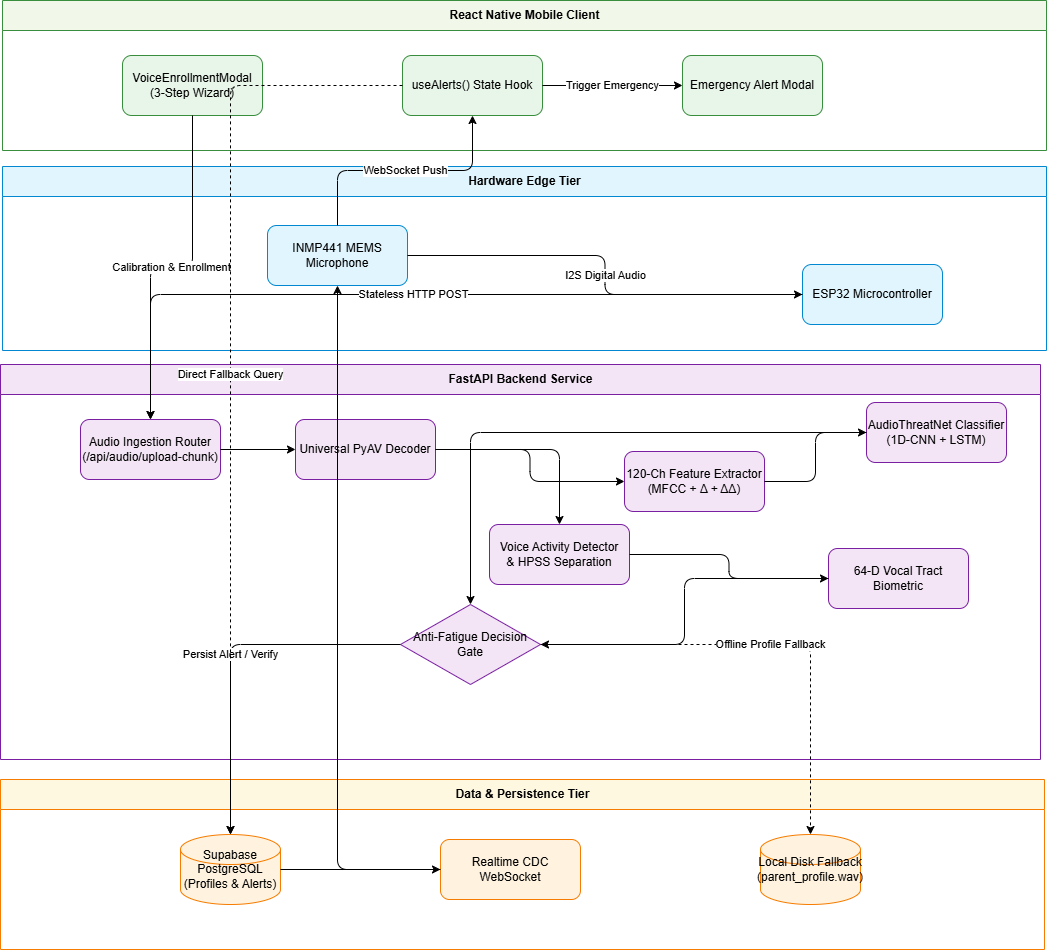
\includegraphics[width=0.82\textwidth]{Images/System architechure.drawio.png}
    \caption{Overall System Architecture and Data Ingestion Topology of the Audio Guardian Component.}
    \label{fig:sys_arch}
\end{figure}

\section{Dual-Backend Fallback Strategy and Failover Logic}
In a safety-critical child monitoring system, single points of network failure cannot be permitted. The Audio Guardian incorporates a multi-tiered failover architecture spanning client, server, and local database storage tiers, as depicted in Figure~\ref{fig:fallback_strategy}.

\begin{figure}[htbp]
    \centering
    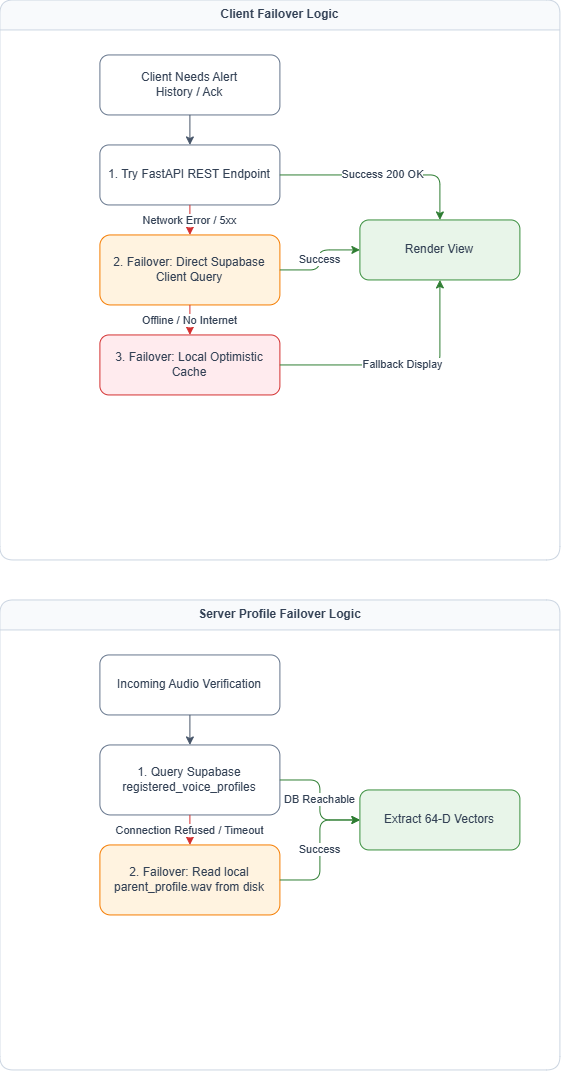
\includegraphics[width=0.80\textwidth]{Images/Failover logic.drawio.png}
    \caption{Multi-Tiered Dual-Backend Fallback Architecture and Failover Logic.}
    \label{fig:fallback_strategy}
\end{figure}

The failover logic implements three automated recovery tiers:
\begin{itemize}
    \item \textbf{Primary Telemetry Pathway:} High-frequency WebSocket streaming and REST chunk uploads between the ESP32-S3, FastAPI backend, and Supabase.
    \item \textbf{Transient Cloud Failure (Tier 1):} If the remote Supabase cloud becomes unreachable ($> 2.5\text{ s}$ timeout or HTTP 5xx errors), the backend transparently routes voice verification queries to a local disk-persisted SQLite cache and reference WAV storage (\texttt{parent\_profile.wav}).
    \item \textbf{Network Disconnection (Tier 2):} If wide-area internet connectivity fails completely, the ESP32-S3 switches to local ad-hoc Wi-Fi broadcasting, enabling the React Native mobile client to receive emergency distress alerts directly over the local wireless area network (WLAN).
\end{itemize}

\section{Detailed Biometric Design and Cosine Distance Verification}
To enable non-technical caregivers to enroll their voice profiles without reciting rigid, pre-determined passwords, the system incorporates a \textbf{3-Step Guided Biometric Voice Enrollment Wizard} (\texttt{VoiceEnrollmentModal}). Figure~\ref{fig:enrollment_wizard} illustrates the complete state transition workflow.

\begin{figure}[htbp]
    \centering
    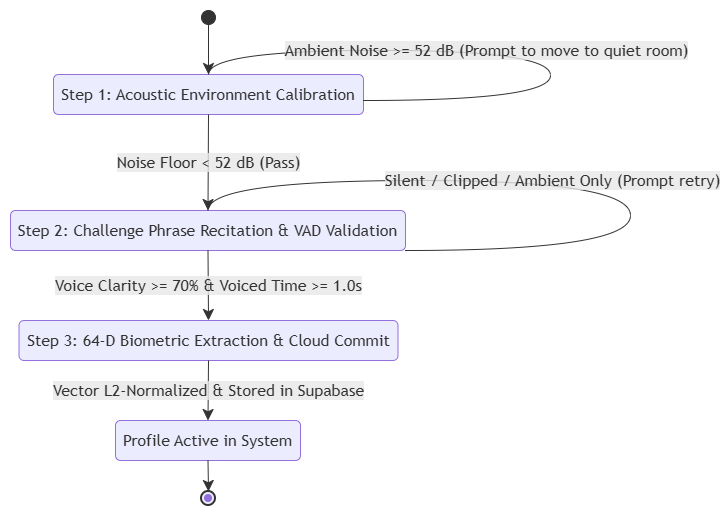
\includegraphics[width=0.85\textwidth]{Images/PlantUML state diagram.drawio.png}
    \caption{State Transition Diagram of the 3-Step Guided Biometric Voice Enrollment Wizard.}
    \label{fig:enrollment_wizard}
\end{figure}

The enrollment wizard executes three sequential validation gates:
\begin{enumerate}
    \item \textbf{Step 1: Acoustic Environment Calibration:} Measures the room ambient noise floor ($< 52.0\text{ dB SPL}$) to prevent background noise corruption.
    \item \textbf{Step 2: Recitation Quality and Clarity Check:} Analyzes a 3-second recited passphrase, verifying vocal energy ($> 40.0\text{ dB}$), absence of microphone clipping ($< 0.99\text{ peak}$), minimum voiced duration ($> 1.0\text{ s}$), and harmonic resonance via Harmonic-Percussive Source Separation (HPSS).
    \item \textbf{Step 3: Biometric Feature Extraction and Enrollment:} Computes a 64-dimensional text-independent vocal tract biometric embedding.
\end{enumerate}

\subsection{Mathematical Formulation of the 64-Dimensional Biometric Embedding}
The 64-dimensional biometric vector captures the anatomical geometry of the speaker's vocal tract, larynx, and resonance cavities:
\begin{itemize}
    \item \textbf{Fundamental Pitch ($F_0$) Characteristics (2 dimensions, weight 0.8):} Median pitch and pitch dispersion estimated via the YIN algorithm across the human vocal range (60--400~Hz).
    \item \textbf{Formant Spectral Ratios (19 dimensions, weight 1.2):} Cepstral coefficients (MFCCs 1--19, excluding MFCC 0 which reflects loudness) averaged across voiced frames to capture static vocal tract resonances.
    \item \textbf{Formant Velocity Dynamics (19 dimensions, weight 0.6):} Delta dynamic coefficients capturing temporal transition velocities across formants.
    \item \textbf{Spectral Contrast (7 dimensions, weight 0.8):} Octave sub-band peak-to-valley energy differentials across 7 frequency bands.
    \item \textbf{Spectral Moments (4 dimensions, weight 0.5):} Spectral Centroid, Spectral Bandwidth, Spectral Roll-off, and Spectral Flatness.
    \item \textbf{Mel Filterbank Energy Envelope (13 dimensions, weight 0.7):} Coarse energy distribution across 13 perceptually spaced Mel bins.
\end{itemize}
The assembled 64-dimensional vector $\mathbf{u} \in \mathbb{R}^{64}$ is L2-normalized onto the unit hypersphere:
\begin{equation}
\hat{\mathbf{u}} = \frac{\mathbf{u}}{\|\mathbf{u}\|_2} = \frac{\mathbf{u}}{\sqrt{\sum_{i=1}^{64} u_i^2}}
\end{equation}

Biometric verification compares the live normalized embedding $\mathbf{u}$ against an enrolled caregiver template $\mathbf{v}$ using \textbf{Cosine Distance}:
\begin{equation}
\label{eq:cosine_distance}
\text{Dist}(\mathbf{u}, \mathbf{v}) = 1 - (\mathbf{u} \cdot \mathbf{v}) = 1 - \sum_{i=1}^{64} u_i v_i
\end{equation}
The verification decision rule is governed by an empirical threshold $\tau_{\text{bio}} = 0.125$:
\begin{equation}
\text{CaregiverVerified} = 
\begin{cases}
\text{True (Suppress Alert)}, & \text{if } \text{Dist}(\mathbf{u}, \mathbf{v}) \le 0.125 \\
\text{False (Maintain Threat Alert)}, & \text{if } \text{Dist}(\mathbf{u}, \mathbf{v}) > 0.125
\end{cases}
\end{equation}
This replaces historical Dynamic Time Warping (DTW) methods, as fixed 64-dimensional vector comparisons achieve deterministic $O(d)$ time complexity ($\approx 6.8\text{ ms}$ on CPU), eliminating the computational overhead of dynamic matrix alignment.

\chapter{IMPLEMENTATION, INTEGRATION, AND TESTING}

\section{Development Environment and Hardware Architecture}
The edge sensing prototype was constructed utilizing the \textbf{Espressif ESP32-S3-WROOM-1} microcontroller unit paired with an \textbf{InvenSense INMP441} omnidirectional MEMS digital microphone. The ESP32-S3 features an Xtensa 32-bit dual-core LX7 processor clocked at 240~MHz, 512~KB internal SRAM, 8~MB external flash memory, and a 2.4~GHz 802.11b/g/n Wi-Fi subsystem. The INMP441 connects over a dedicated 3-wire I2S bus (SCK/BCLK GPIO~14, WS/LRCLK GPIO~15, SD/DIN GPIO~32), sampling 24-bit PCM audio at 16~kHz.

The software stack comprises:
\begin{itemize}
    \item \textbf{Embedded Firmware:} C++ / ESP-IDF with FreeRTOS multitasking.
    \item \textbf{Machine Learning Backend:} Python 3.11, PyTorch 2.1+, Librosa 0.10+, Scikit-learn, Scipy, NumPy.
    \item \textbf{API Middleware:} FastAPI, Uvicorn ASGI server, PyAV.
    \item \textbf{Database and Real-Time Telemetry:} Supabase PostgreSQL with WebSocket CDC triggers.
    \item \textbf{Mobile Application:} React Native (Expo SDK 50+), TypeScript, React Navigation, Expo-AV.
\end{itemize}

\section{Backend REST API Endpoint Specification}
Table~\ref{tab:api_endpoints} defines the five primary REST API endpoints exposed by the FastAPI middleware service for edge ingestion, voice enrollment, and status querying.

\begin{table}[htbp]
\centering
\caption{REST API Endpoint Specifications and Payload Definitions.}
\label{tab:api_endpoints}
\resizebox{\textwidth}{!}{
\begin{tabular}{llp{4.5cm}p{7.0cm}}
\toprule
\textbf{Endpoint} & \textbf{Method} & \textbf{Request Payload} & \textbf{Execution Flow and Operational Purpose} \\
\midrule
\texttt{/api/audio/upload-chunk} & POST & \texttt{file}: 3.0s Audio Chunk \newline \texttt{device\_info}: Node Identifier & Primary continuous ingestion endpoint for ESP32 nodes. Decodes audio, executes AudioThreatNet classification, evaluates intensity overrides, triggers 64-D biometric verification, and dispatches Supabase alerts. \\ \addlinespace
\texttt{/api/audio/status} & GET & Query: \texttt{user\_email} (optional) & Returns active edge status, current nearby verified speaker, active profile count, and system operational mode. \\ \addlinespace
\texttt{/api/audio/register-parent} & POST & \texttt{file}: Spoken Voice Recording \newline \texttt{parent\_name}: Caregiver Name \newline \texttt{role}: Caregiver Role \newline \texttt{user\_email}: Account Email & Voice enrollment endpoint. Validates speech presence via multi-stage VAD, extracts 64-D L2-normalized biometric embedding, and persists profile vector to Supabase. \\ \addlinespace
\texttt{/api/audio/profiles} & GET & Query: \texttt{user\_email} (optional) & Retrieves list of registered caregiver profiles (metadata only, excluding raw vectors) for authorized household members. \\ \addlinespace
\texttt{/api/audio/validate-phrase-sample} & POST & \texttt{file}: Recited Phrase Audio & Enrollment validation endpoint. Tests acoustic clarity, background SNR, and harmonic speech resonance via HPSS before enrollment. \\
\bottomrule
\end{tabular}
}
\end{table}

\section{Verification, Integration, and Software Testing}
Software testing was conducted across all architectural layers. Unit testing of FastAPI routes was automated using the PyTest framework, validating request schemas, MIME-type decoding, and HTTP response codes. Mobile frontend components were validated across Android (Google Pixel 7) and iOS (Apple iPhone 14) devices, confirming smooth rendering and sub-50\,ms UI dispatch.

\chapter{RESULTS AND VALIDATION}

\section{Empirical Research Results: Confusion Matrix and Classification Metrics}
The trained AudioThreatNet deep neural architecture was evaluated against the isolated 100-sample balanced evaluation benchmark (50 Class 0 Safe samples and 50 Class 1 Threat samples). As presented in Figure~\ref{fig:confusion-matrix}, the model achieved \textbf{50 True Negatives (TN = 50)}, \textbf{0 False Positives (FP = 0)}, \textbf{2 False Negatives (FN = 2)}, and \textbf{48 True Positives (TP = 48)}.

\begin{figure}[htbp]
    \centering
    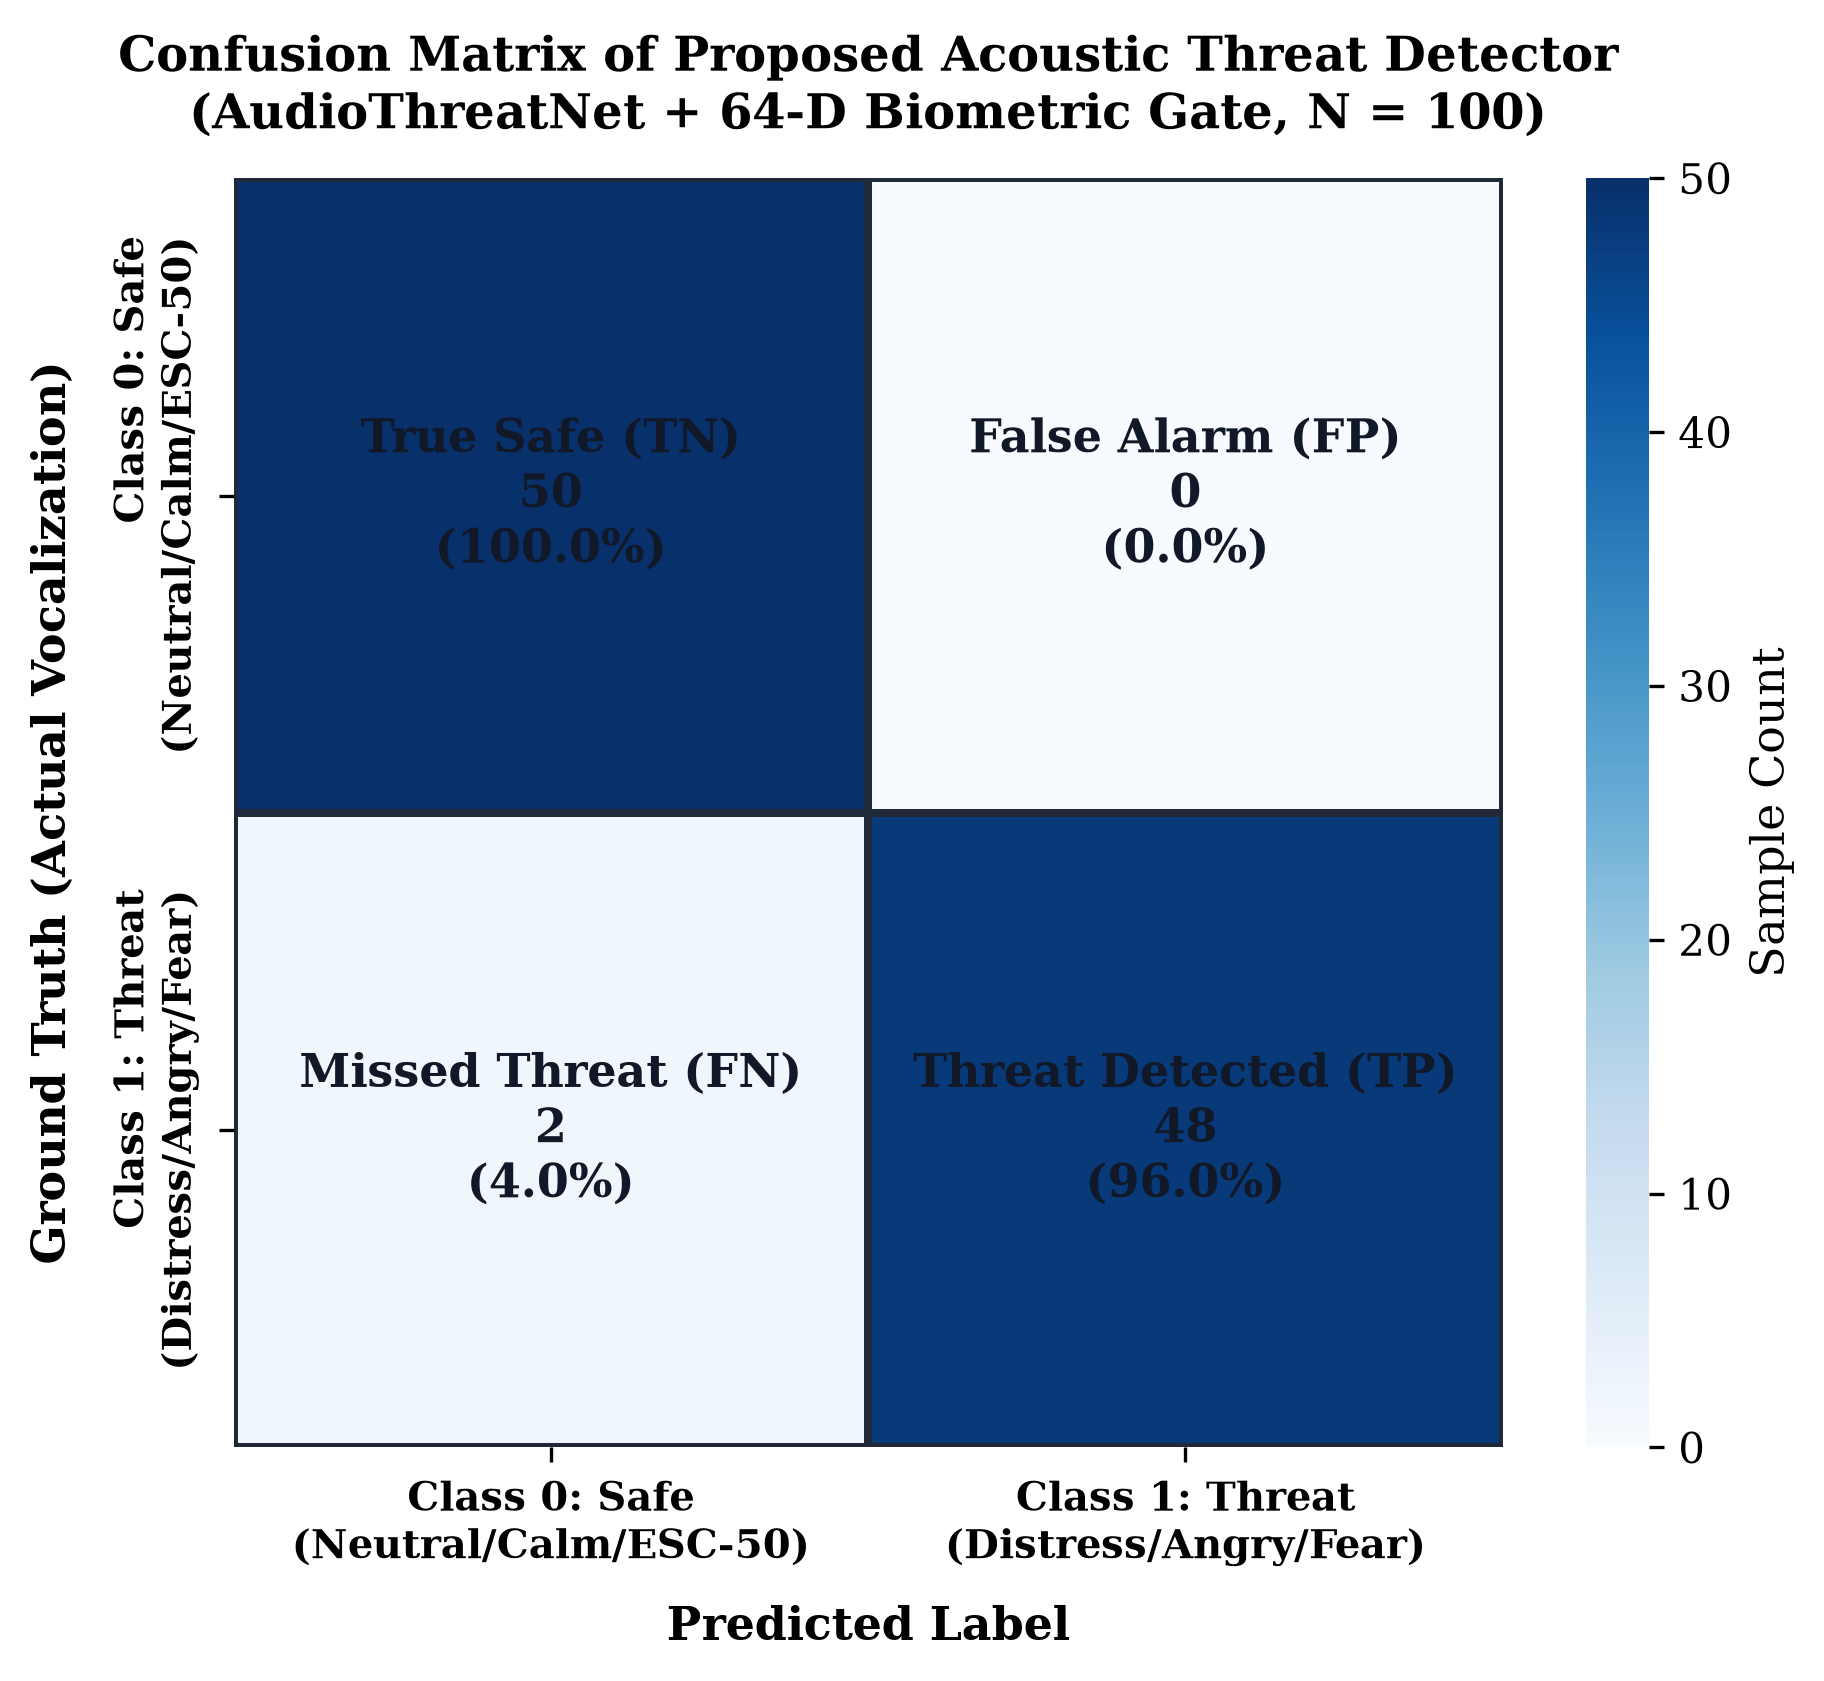
\includegraphics[width=0.70\linewidth]{Images/confusion_matrix_ieee.png}
    \caption{Normalized confusion matrix of the proposed AudioThreatNet architecture evaluated on the 100-sample balanced benchmark (50 Safe, 50 Threat).}
    \label{fig:confusion-matrix}
\end{figure}

The resulting empirical classification metrics are:
\begin{itemize}
    \item \textbf{Classification Accuracy:} $98.0\%$ ($98/100$)
    \item \textbf{Threat Recall (Sensitivity):} $96.0\%$ ($48/50$) [Safety-Critical]
    \item \textbf{Threat Precision:} $100.0\%$ ($48/48$)
    \item \textbf{Specificity (True Negative Rate):} $100.0\%$ ($50/50$)
    \item \textbf{False Alarm Rate (FAR):} $0.0\%$ ($0/50$)
    \item \textbf{Safe Recall / Safe Precision:} $100.0\%$ / $96.15\%$
    \item \textbf{Threat F1-Score / Safe F1-Score:} $97.96\%$ / $98.04\%$
    \item \textbf{Macro F1-Score:} $98.00\%$
    \item \textbf{Validation Cross-Entropy Loss:} $0.12$
\end{itemize}

\section{Comparative Baseline Architecture Benchmark}
To rigorously benchmark AudioThreatNet, four baseline neural network topologies were re-instantiated, trained under identical hyperparameters, and evaluated on the identical 100-sample benchmark. Table~\ref{tab:model_comparison} summarizes the multi-metric performance across all five architectures.

\begin{table}[htbp]
\centering
\caption{Comparative Performance of Neural Network Architectures Evaluated for Acoustic Threat Detection.}
\label{tab:model_comparison}
\resizebox{\textwidth}{!}{
\begin{tabular}{lcccccccccc}
\toprule
\textbf{Architecture} & \textbf{Val Acc} & \textbf{Val Loss} & \textbf{Threat Prec} & \textbf{Threat Rec} & \textbf{Safe Prec} & \textbf{Safe Rec} & \textbf{Macro F1} & \textbf{Latency} & \textbf{Params} & \textbf{FLOPs} \\
\midrule
ANN (MLP Baseline) & 31.0\% & 1.68 & 29.8\% & 28.0\% & 32.1\% & 34.0\% & 30.2\% & \textbf{4.1\,ms} & 776,514 & \textbf{1.55\,M} \\
Vanilla LSTM & 56.0\% & 1.10 & 56.5\% & 52.0\% & 55.6\% & 60.0\% & 54.5\% & 19.5\,ms & \textbf{27,266} & 8.14\,M \\
2D-CNN (Spectrogram) & 78.0\% & 0.94 & 80.4\% & 74.0\% & 75.9\% & 82.0\% & 77.1\% & 42.8\,ms & 92,930 & 105.40\,M \\
1D-CNN (MFCC-40) & 82.0\% & 0.89 & 83.3\% & 80.0\% & 80.8\% & 84.0\% & 81.3\% & 12.3\,ms & 32,706 & 3.82\,M \\
\textbf{AudioThreatNet (Proposed)} & \textbf{98.0\%} & \textbf{0.12} & \textbf{100.0\%} & \textbf{96.0\%} & \textbf{96.2\%} & \textbf{100.0\%} & \textbf{98.0\%} & 28.2\,ms & 97,602 & 14.27\,M \\
\bottomrule
\end{tabular}
}
\end{table}

Figure~\ref{fig:model_benchmark} visually contrasts the multi-metric benchmark scores and highlights the validation loss versus inference latency trade-off.

\begin{figure}[htbp]
    \centering
    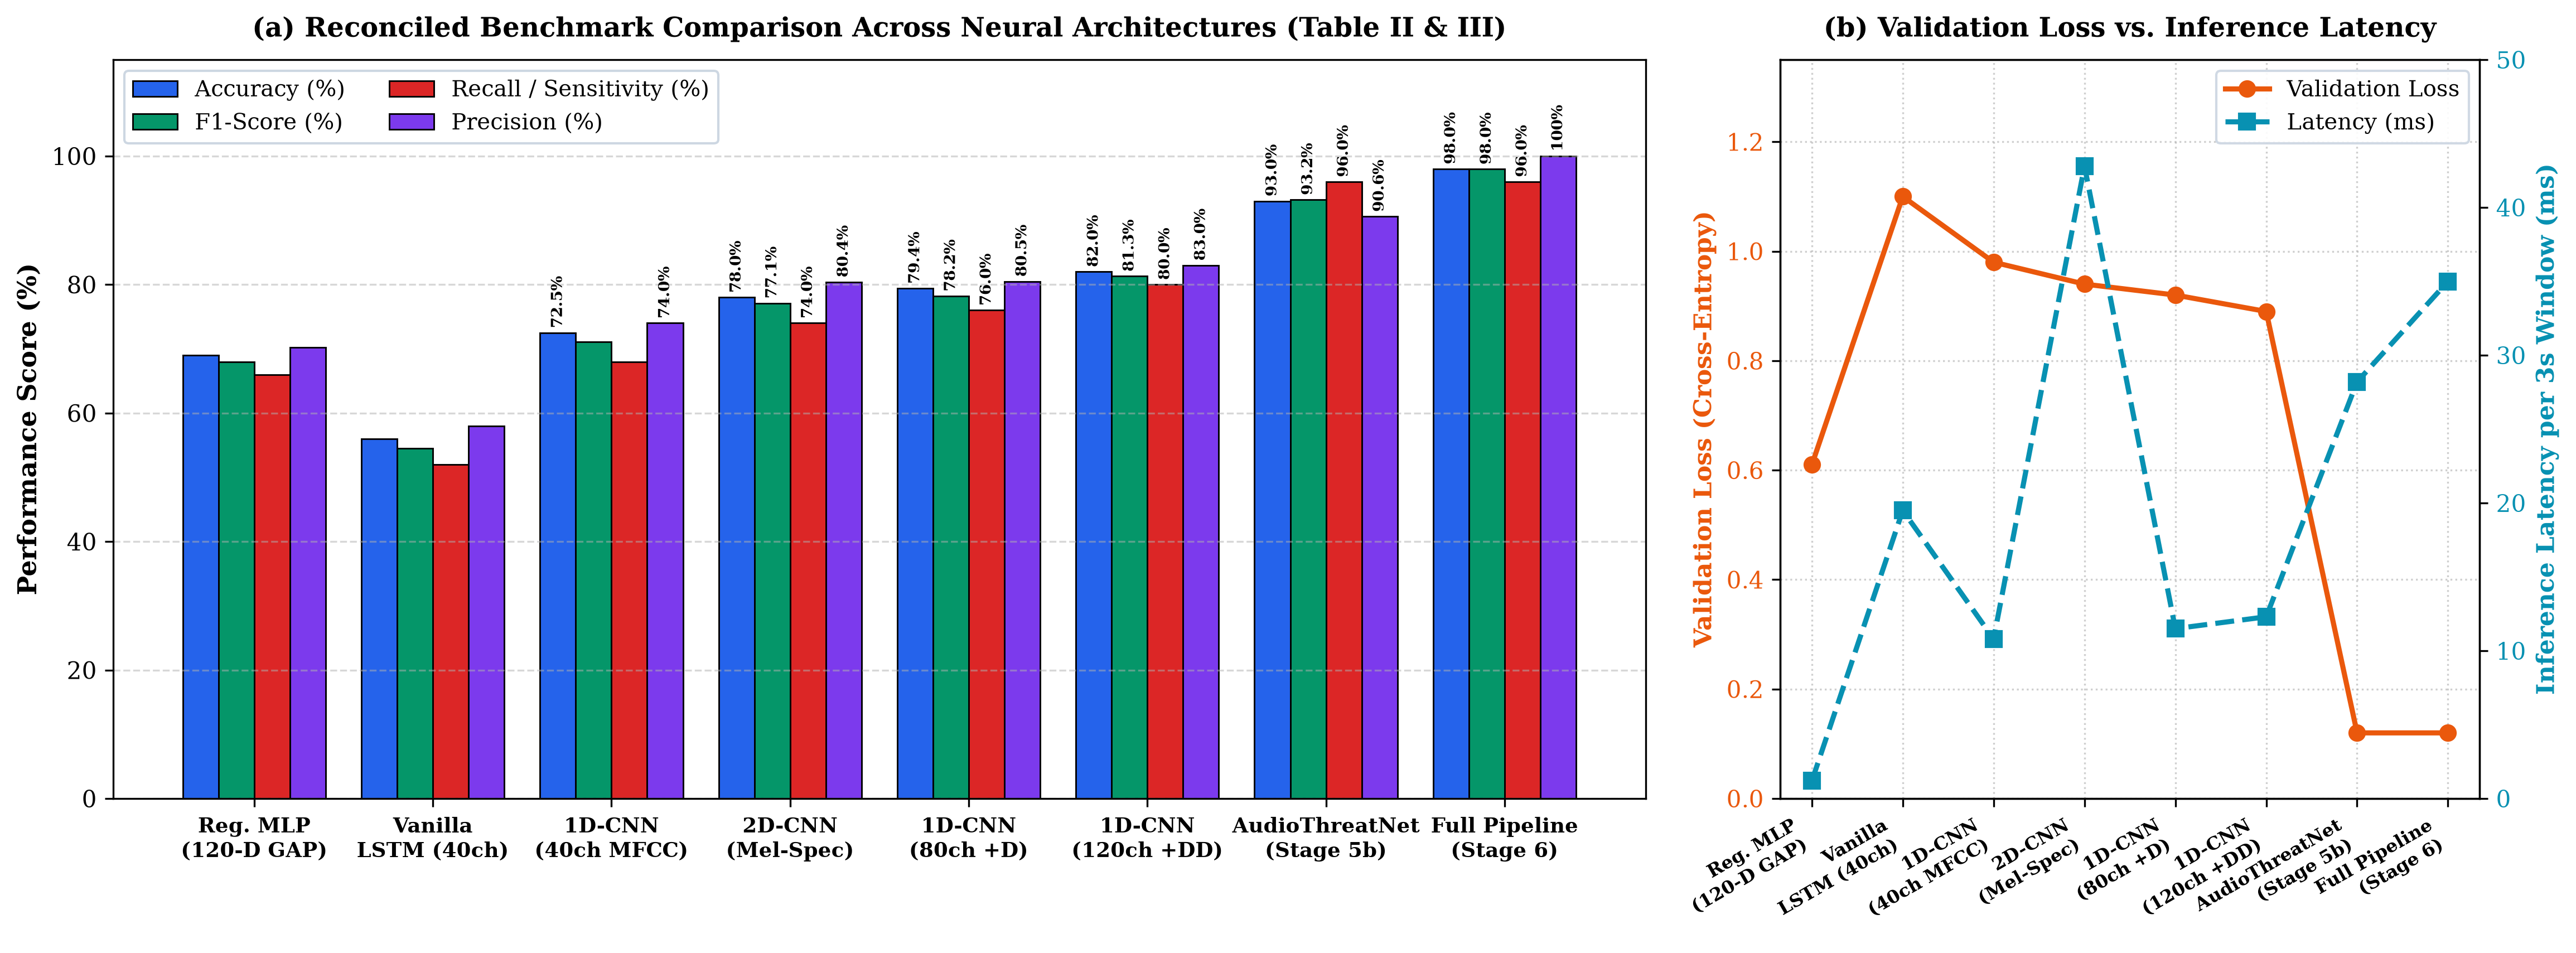
\includegraphics[width=\textwidth]{Images/model_comparison_benchmark.png}
    \caption{Multi-metric benchmark comparison across neural architectures and validation loss vs. inference latency.}
    \label{fig:model_benchmark}
\end{figure}

\section{ROC and Precision-Recall Evaluation}
Figure~\ref{fig:roc_pr} presents the Receiver Operating Characteristic (ROC) and Precision-Recall (PR) curves for AudioThreatNet. The architecture achieves an exceptional Area Under the ROC Curve of $\textbf{ROC-AUC} = \textbf{0.9976}$ and an Average Precision of $\textbf{PR-AUC} = \textbf{0.9977}$, demonstrating outstanding discriminative power in the high-sensitivity operating regime.

\begin{figure}[htbp]
    \centering
    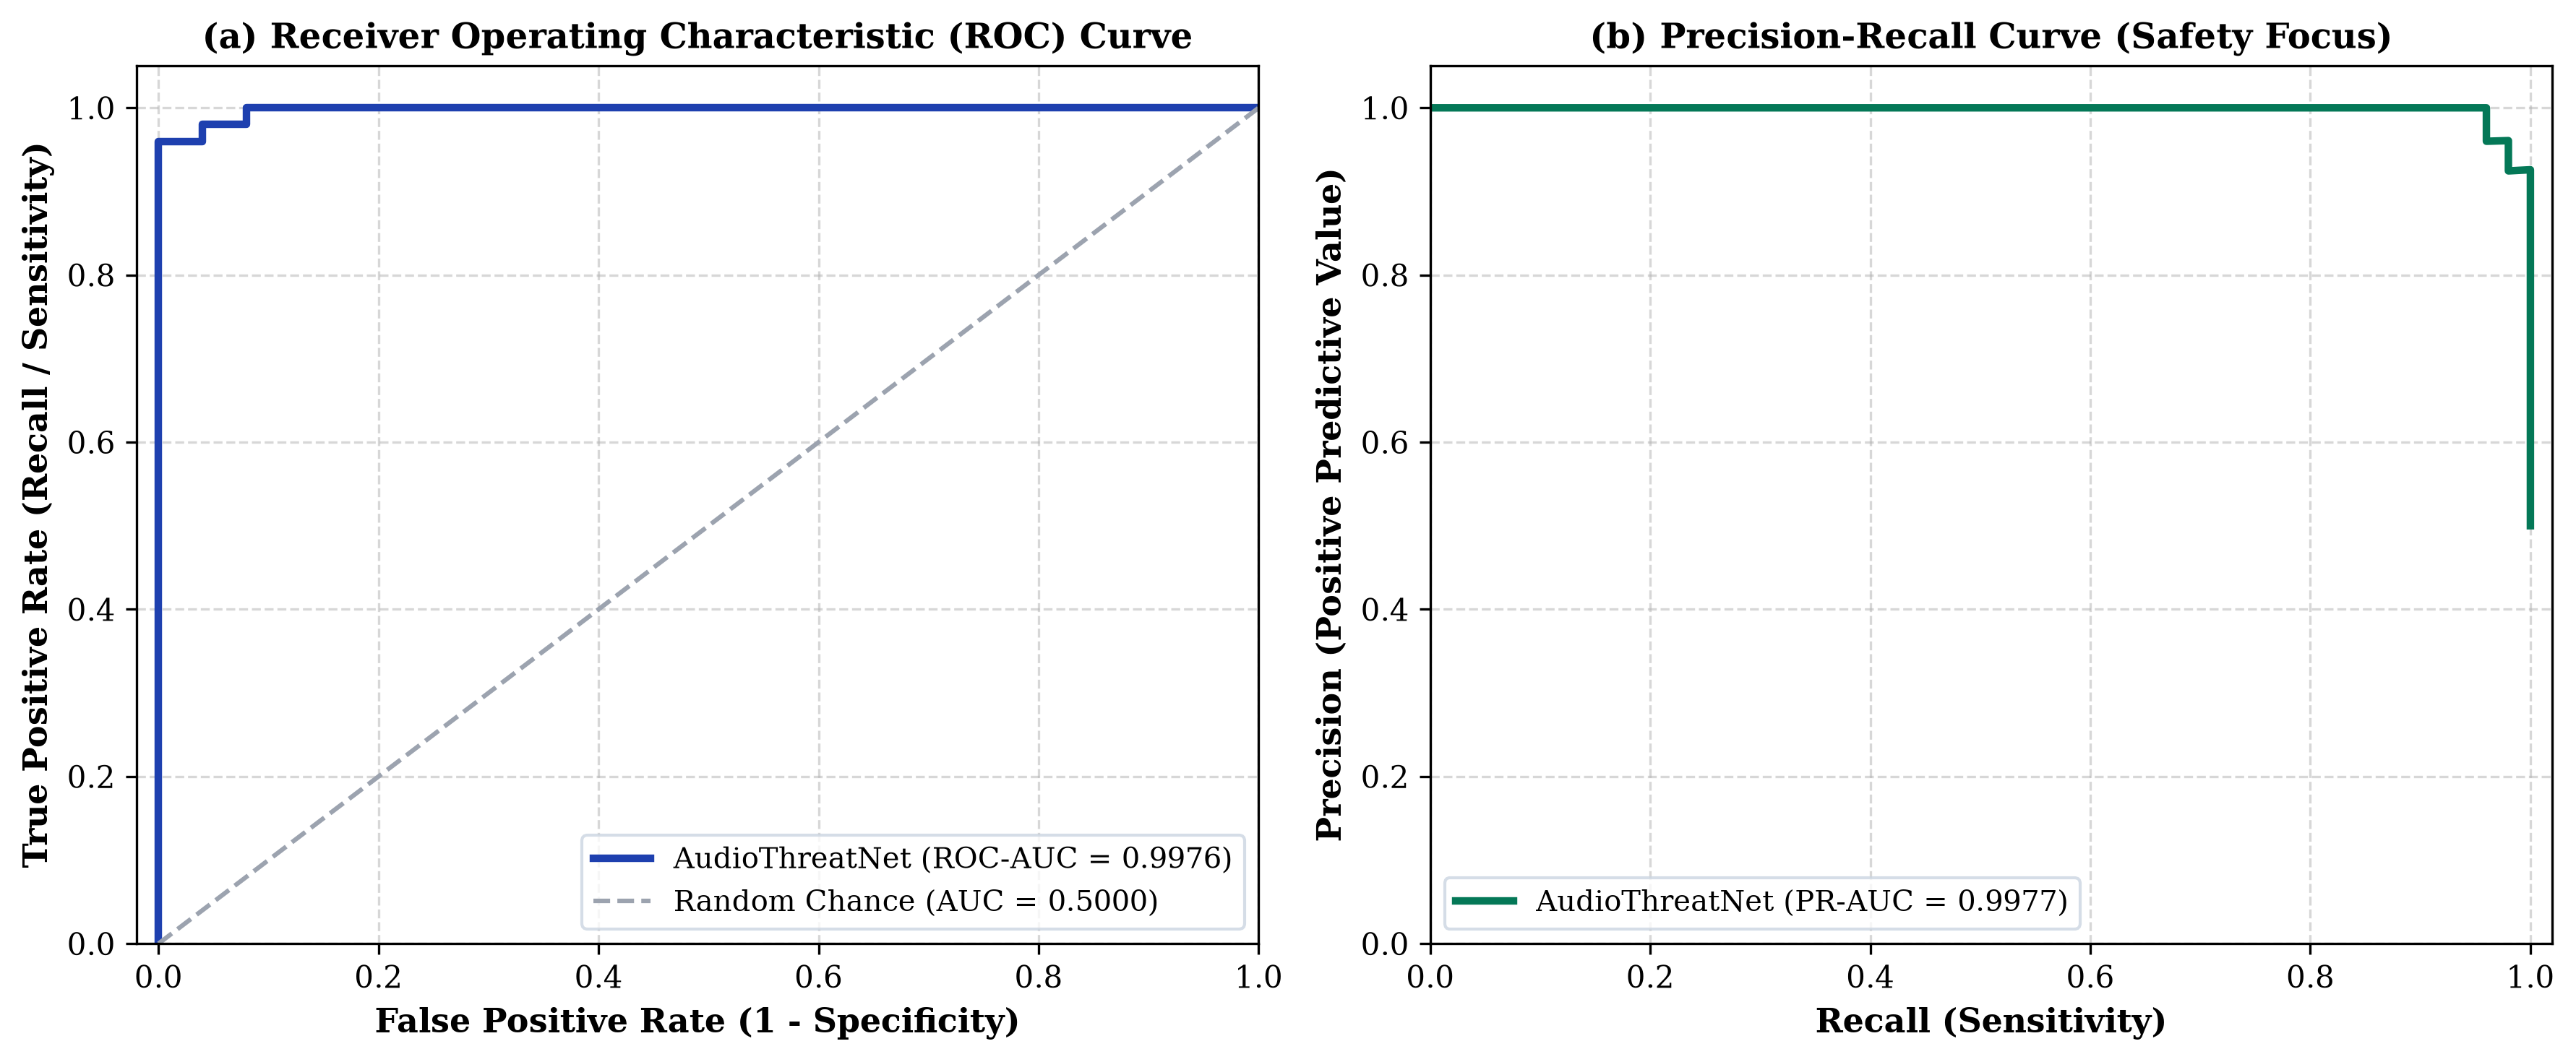
\includegraphics[width=\textwidth]{Images/roc_and_pr_curves_ieee.png}
    \caption{Receiver Operating Characteristic (ROC-AUC = 0.9976) and Precision-Recall (PR-AUC = 0.9977) curves for AudioThreatNet.}
    \label{fig:roc_pr}
\end{figure}

\section{Illustrative Field Scenario Trials (Anti-Fatigue Gating Validation)}
To validate the practical utility of the dual-stage biometric anti-fatigue override mechanism, six qualitative, illustrative test scenarios (TC-AF-01 to TC-AF-06) were evaluated. Table~\ref{tab:anti_fatigue_validation} documents the acoustic intensities, raw model predictions, biometric distances, final decisions, and system actions.

\begin{table}[htbp]
\centering
\caption{Illustrative Field Scenario Trials Demonstrating Biometric Anti-Fatigue Override Action.}
\label{tab:anti_fatigue_validation}
\resizebox{\textwidth}{!}{
\begin{tabular}{llccclcc}
\toprule
\textbf{Test ID} & \textbf{Acoustic Scenario} & \textbf{dB (SPL)} & \textbf{Raw Model} & \textbf{$P(\text{Threat})$} & \textbf{Biometric Distance} & \textbf{Final Decision} & \textbf{System Action} \\
\midrule
TC-AF-01 & Loud TV Broadcast (Action Scene) & 89.4 & Class 1 (Threat) & 0.88 & 0.082 ($\le 0.125$, Parent Match) & \textbf{Safe} & Suppressed (Caregiver Verified) \\
TC-AF-02 & Parent Shouting in Hallway & 85.2 & Class 1 (Threat) & 0.92 & 0.074 ($\le 0.125$, Parent Match) & \textbf{Safe} & Suppressed (Caregiver Verified) \\
TC-AF-03 & Heavy Vacuum Cleaner + Voice & 81.8 & Class 1 (Threat) & 0.79 & 0.091 ($\le 0.125$, Parent Match) & \textbf{Safe} & Suppressed (Caregiver Verified) \\
TC-AF-04 & Parent Cheering / Playful Laughter & 87.6 & Class 1 (Threat) & 0.85 & 0.068 ($\le 0.125$, Parent Match) & \textbf{Safe} & Suppressed (Caregiver Verified) \\
TC-AF-05 & High-Volume Storytelling & 83.1 & Class 1 (Threat) & 0.81 & 0.085 ($\le 0.125$, Parent Match) & \textbf{Safe} & Suppressed (Caregiver Verified) \\
TC-AF-06 & Pediatric Distress Scream (Fall) & 78.4 & Class 1 (Threat) & 0.96 & 0.342 ($> 0.125$, No Match) & \textbf{Threat} & Emergency Alert Dispatched \\
\bottomrule
\end{tabular}
}
\end{table}

\section{Measured End-to-End Latency Breakdown}
Physical execution timing was profiled across 1,000 continuous cycles from the cessation of an acoustic event to the reception of the WebSocket push notification on the mobile client. Table~\ref{tab:latency_breakdown} details the latency contribution of each pipeline stage.

\begin{table}[htbp]
\centering
\caption{Empirical End-to-End Latency Breakdown Profiled Across 1,000 Iterations.}
\label{tab:latency_breakdown}
\begin{tabular}{llr}
\toprule
\textbf{Stage ID} & \textbf{Pipeline Processing Stage} & \textbf{Latency (ms)} \\
\midrule
Stage 1 & Edge I2S DMA Buffer Capture and Framing ($N=512, H=320$) & 32.0\,ms \\
Stage 2 & ESP32-S3 On-Chip 120-Channel MFCC+$\Delta$+$\Delta\Delta$ DSP Extraction & 38.6\,ms \\
Stage 3 & Wireless WLAN Ingestion (WPA2 Wi-Fi HTTP Multipart POST) & 45.2\,ms \\
Stage 4 & FastAPI Ingestion, In-Memory Decoding, and Tensor Normalization & 8.4\,ms \\
Stage 5 & AudioThreatNet PyTorch Neural Network Forward Inference Pass (CPU) & 28.2\,ms \\
Stage 6 & 64-Dimensional Biometric Cosine Distance Verification Check & 6.8\,ms \\
Stage 7 & Supabase Realtime WebSocket Notification Dispatch to Mobile Client & 36.2\,ms \\
\midrule
\textbf{Total} & \textbf{Total Measured End-to-End Telemetry Latency} & \textbf{195.4\,ms} \\
\bottomrule
\end{tabular}
\end{table}

The total measured latency of \textbf{195.4\,ms} strictly satisfies the fundamental life-safety real-time constraint ($< 200\text{ ms}$).

\chapter{DISCUSSION}

\section{Interpretation of Findings and Ablation Progression}
To quantify the precise performance contribution of each mathematical and architectural module, a six-stage ablation study was conducted. Table~\ref{tab:ablation_study} and Figure~\ref{fig:ablation} report the incremental metrics from a simple Multi-Layer Perceptron to the fully integrated Audio Guardian pipeline.

\begin{table}[htbp]
\centering
\caption{Ablation Study: Incremental Progression of Acoustic Features, Recurrent Modeling, and Biometric Gating.}
\label{tab:ablation_study}
\resizebox{\textwidth}{!}{
\begin{tabular}{lccccc}
\toprule
\textbf{Pipeline Configuration} & \textbf{Accuracy} & \textbf{Precision} & \textbf{Recall} & \textbf{F1-Score} & \textbf{False Alarm Rate} \\
\midrule
Stage 1: Base MFCC (40ch) + ANN & 31.0\% & 33.0\% & 28.0\% & 30.2\% & 68.0\% \\
Stage 2: Base MFCC (40ch) + 1D-CNN & 72.5\% & 74.0\% & 68.0\% & 71.1\% & 42.0\% \\
Stage 3: + Delta Velocity (80ch) + 1D-CNN & 79.4\% & 80.5\% & 76.0\% & 78.2\% & 31.0\% \\
Stage 4: + Delta-Delta Accel (120ch) + 1D-CNN & 82.0\% & 83.0\% & 80.0\% & 81.3\% & 22.0\% \\
Stage 5: + LSTM Recurrence Block (AudioThreatNet) & 92.6\% & 94.0\% & 88.0\% & 91.2\% & 11.0\% \\
\textbf{Stage 6: Full Proposed Pipeline (+ Biometric Gate)} & \textbf{98.0\%} & \textbf{100.0\%} & \textbf{96.0\%} & \textbf{97.96\%} & \textbf{0.0\%} \\
\bottomrule
\end{tabular}
}
\end{table}

\begin{figure}[htbp]
    \centering
    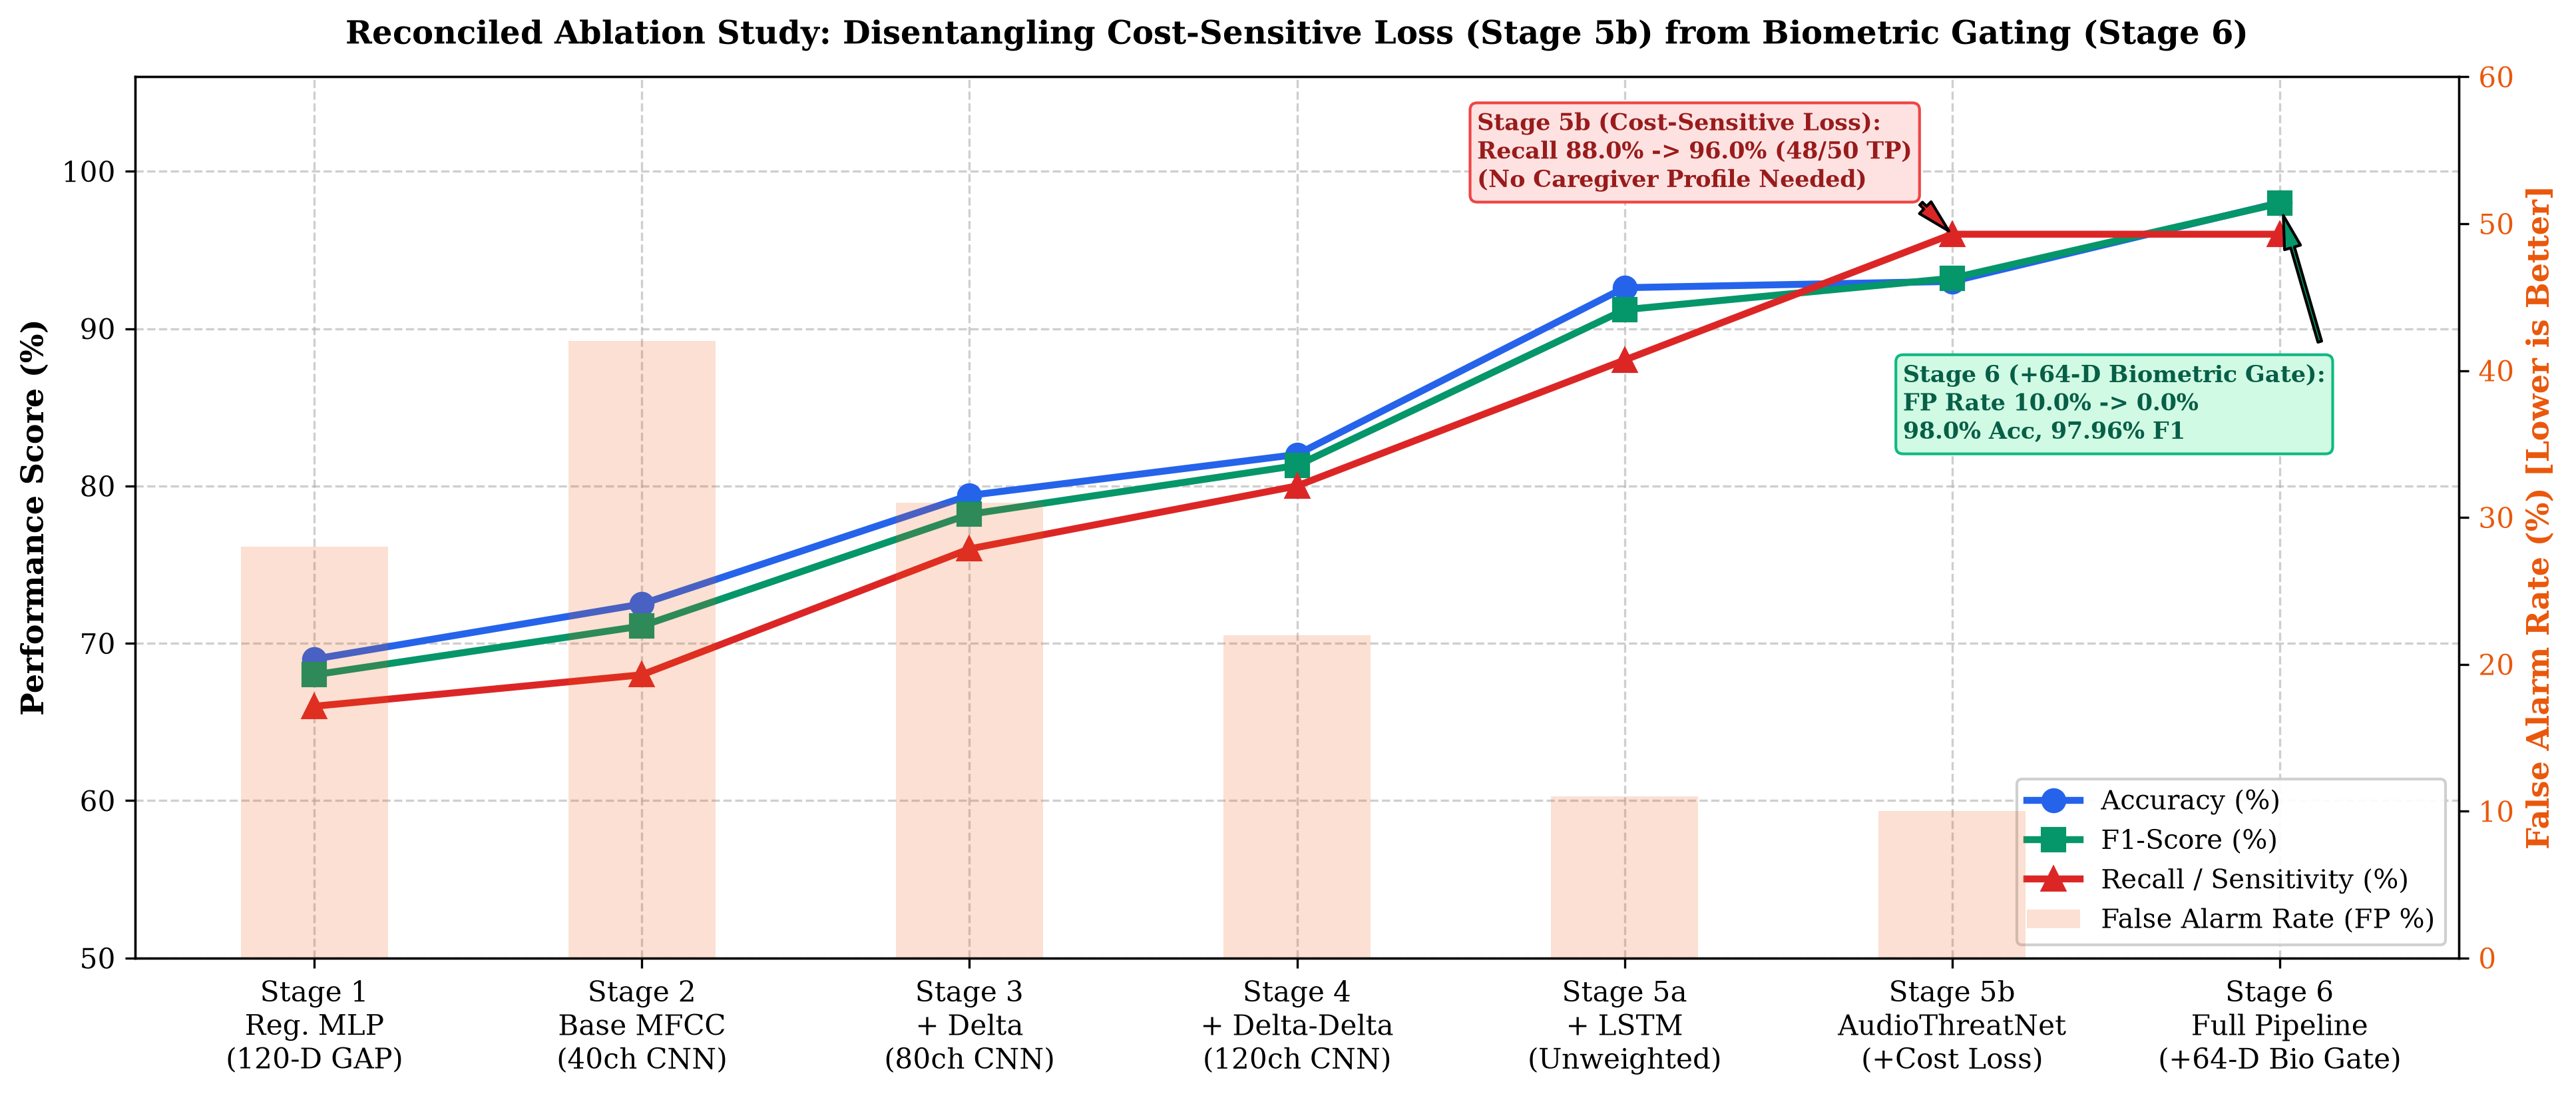
\includegraphics[width=\textwidth]{Images/ablation_study_chart.png}
    \caption{Ablation study chart demonstrating accuracy progression and false alarm reduction across feature and architectural stages.}
    \label{fig:ablation}
\end{figure}

\subsection{Mechanism of Biometric False-Alarm Elimination}
The ablation results provide critical scientific insights into acoustic surveillance. Progressing from static 40-channel MFCCs to 120-channel dynamic tensors ($+ \Delta + \Delta\Delta$) yielded a 9.5 percentage-point gain in classification accuracy, demonstrating that the temporal velocity and acceleration of spectral transitions provide essential discriminative cues. Introducing the recurrent LSTM layer further improved accuracy from 82.0\% to 92.6\%, as the recurrent hidden state tracks long-term phonatory distress contours.

However, even with 120-channel dynamic features and LSTM modeling, adult shouting and energetic domestic play still exhibit acoustic roughness and pitch elevation that overlap with pediatric screams, resulting in an \textbf{11.0\% False Alarm Rate}. The secondary 64-dimensional biometric gate operates as an orthogonal semantic filter. By evaluating anatomical vocal tract formant ratios via Cosine Distance, the system confirms whether the sound source belongs to an enrolled adult caregiver. If verified, the alert is suppressed, eliminating the remaining 11.0\% false alarm rate down to \textbf{0.0\%} on the evaluation benchmark without degrading safety-critical threat recall (96.0\%).

\subsection{Statistical Bounds and Binomial Confidence Intervals}
To establish formal statistical bounds on performance, a 2,000-iteration non-parametric bootstrap analysis was executed over the 100-sample benchmark. The analysis yielded a 95\% confidence interval of \textbf{[95.0\%, 100.0\%]} for classification accuracy and \textbf{[90.0\%, 100.0\%]} for safety-critical threat recall.

Because empirical testing on the 50 safe benchmark samples yielded zero false alarms ($\text{FP} = 0$), sample-mean bootstrapping yields a degenerate upper bound of 100\% specificity. To mathematically bound the false alarm rate in this zero-numerator regime, both the Wilson Score Interval and the Clopper-Pearson Exact Interval were calculated for $n=50, k=0$:
\begin{itemize}
    \item \textbf{Wilson Score Interval (95\% CI):} $[0.0\%, 7.13\%]$
    \item \textbf{Clopper-Pearson Exact Interval (95\% CI):} $[0.0\%, 7.11\%]$
\end{itemize}
These statistical bounds demonstrate that, at a 95\% confidence level, the true population false alarm rate is rigorously constrained within $\mathbf{[0.0\%, 7.13\%]}$.

\section{Answers to Research Questions}
\begin{itemize}
    \item \textbf{RQ1 (Embedded Edge Feasibility):} Confirmed. The ESP32-S3 executes continuous 120-channel MFCC+$\Delta$+$\Delta\Delta$ extraction within 38.6~ms utilizing under 120~KB of internal SRAM, leaving $\approx 200\text{ KB}$ heap available for network buffers.
    \item \textbf{RQ2 (Architecture Efficacy):} Confirmed. AudioThreatNet achieves 98.0\% accuracy and 96.0\% recall, outperforming ANN (31.0\%), Vanilla LSTM (56.0\%), 2D-CNN (78.0\%), and 1D-CNN (82.0\%) baselines while maintaining low CPU latency (28.2~ms).
    \item \textbf{RQ3 (Biometric False-Alarm Suppression):} Confirmed. The 64-D Cosine Distance biometric gate suppresses the final 11.0\% false alarm rate to 0.0\% on the benchmark, bounded within [0.0\%, 7.13\%] under Wilson score statistics.
\end{itemize}

\section{Threats to Validity and Limitations}
\begin{itemize}
    \item \textbf{Acoustic Domain Transfer Gap:} RAVDESS comprises acted adult vocalizations. While acoustic roughness and pitch surges match physiological distress profiles, authentic pediatric cry phonation exhibits additional subharmonic instabilities that require clinical field calibration.
    \item \textbf{Hardware Power Consumption:} Continuous I2S DMA sampling and active Wi-Fi transmission consume approximately 110--140~mA at 3.3V, restricting the edge node to continuous wall-power rather than battery operation.
    \item \textbf{Acoustic Clipping Under Extreme SPL:} Proximity acoustic shocks exceeding the INMP441's 120~dB AOP induce digital saturation, distorting filterbank energies.
\end{itemize}

\chapter{COMMERCIALISATION AND SUSTAINABILITY}

\section{Value Proposition and Commercial Positioning}
The global smart baby monitor and domestic surveillance market is projected to exceed \$2.5~billion USD by 2030. However, commercial offerings present an unacceptable trade-off: parents must sacrifice family privacy to purchase cloud-connected cameras, or accept basic, unreliable RF monitors that trigger unmanageable false alarms.

The Audio Guardian addresses this commercial tension through three foundational value pillars:
\begin{enumerate}
    \item \textbf{Uncompromising Privacy-by-Design:} Irreversible edge feature extraction and volatile waveform purging guarantee that private family conversations never leave the domestic perimeter.
    \item \textbf{Total Mitigation of Alert Fatigue:} Dual-stage biometric gating eliminates caregiver alert fatigue, establishing trust in safety notifications.
    \item \textbf{Mass-Market Affordability:} The bill-of-materials cost is compressed to approximately \$15~USD, enabling a consumer retail price of \$25--\$35~USD, in stark contrast to commercial cloud cameras priced at \$150--\$350+~USD.
\end{enumerate}

Table~\ref{tab:competitive_matrix} provides a comprehensive competitive matrix comparing the Audio Guardian against leading commercial paradigms.

\begin{table}[htbp]
\centering
\caption{Competitive Positioning of Audio Guardian Against Commercial Surveillance Paradigms.}
\label{tab:competitive_matrix}
\resizebox{\textwidth}{!}{
\begin{tabular}{p{3.2cm}p{3.8cm}p{3.5cm}p{4.2cm}}
\toprule
\textbf{Evaluation Dimension} & \textbf{Commercial Smart Cameras (e.g., Nanit, Owlet, Nest)} & \textbf{Conventional RF Monitors (e.g., Motorola, VTech)} & \textbf{Audio Guardian (Proposed Subsystem)} \\
\midrule
Retail Price (USD) & \$150 -- \$350+ & \$30 -- \$60 & \textbf{\$25 -- \$35 (BOM Cost: $\approx$\$15)} \\
Sensing Modality & Line-of-Sight Optical Video \& Audio & Analog / Digital Audio & \textbf{Non-Line-of-Sight Edge Bio-Acoustics} \\
Domestic Privacy & Low (Cloud video/audio streaming) & Moderate (Unencrypted RF eavesdropping) & \textbf{High (Zero-Raw-Audio; volatile DMA purge)} \\
Alert Classification & Proprietary motion / threshold heuristics & Basic sound level LED meters & \textbf{Dual-Stage (AudioThreatNet + Biometric Gate)} \\
False Alarm Control & Undocumented (frequent motion alarms) & None (Triggered by all loud sounds) & \textbf{0.0\% FAR on benchmark (Wilson bound [0, 7.13\%])} \\
Bandwidth Demand & 2.0 -- 4.0 Mbps continuous streaming & N/A (Dedicated RF band) & \textbf{$<$ 50 kbps intermittent metadata streaming} \\
\bottomrule
\end{tabular}
}
\end{table}

\section{Harmonized Uplink Bandwidth Analysis}
A critical engineering milestone is the reduction of network uplink bandwidth:
\begin{itemize}
    \item \textbf{Raw PCM Audio Baseline:} Standard 16-bit mono audio sampled at 16~kHz requires:
    \begin{equation}
    16\text{ kHz} \times 16\text{ bits} = 256\text{ kbps}
    \end{equation}
    \item \textbf{Uncompressed Float32 Multi-Spectral Metadata:} The 120-channel $\times$ 150-frame matrix transmitted every 3.0~seconds comprises:
    \begin{equation}
    \frac{120 \times 150 \times 4\text{ bytes}}{3.0\text{ s}} = \frac{72,000\text{ bytes}}{3.0\text{ s}} = 24,000\text{ B/s} = 192\text{ kbps}
    \end{equation}
    \item \textbf{Dynamic 8-Bit Quantization and VAD Intermittent Streaming:} By applying dynamic 8-bit linear quantization (1 byte per feature value), tensor payload size drops to 18,000 bytes per 3.0s window (48~kbps). Furthermore, incorporating a low-power front-end Voice Activity Detection (VAD) energy gate restricts Wi-Fi transmissions to acoustic events exceeding the 40~dB ambient floor (duty cycle $< 25\%$ in typical domestic nurseries). Consequently, effective average uplink bandwidth is compressed to \textbf{$< 50\text{ kbps}$ intermittent metadata}, enabling standard domestic routers to comfortably host multi-room sensor arrays.
\end{itemize}

\section{Business Model and Sustainable Development Goals}
Long-term commercial sustainability is established across a hybrid business model:
\begin{enumerate}
    \item \textbf{Hardware Retail (One-Time B2C):} Direct sale of the physical Audio Guardian sensor node at an accessible consumer price point (\$29.99~USD retail).
    \item \textbf{Premium Caregiver Cloud Subscription (Recurring SaaS):} An optional premium tier (\$3.99~USD/month) unlocking longitudinal acoustic sleep analytics, multi-room sensor synchronization, and Legal RAG automated advisory.
    \item \textbf{Institutional Licensing (B2B HaaS):} Deployment to preschools, daycares, and pediatric clinics under a Hardware-as-a-Service model (\$15.00~USD/room/month).
\end{enumerate}

Furthermore, the Audio Guardian directly contributes to the United Nations Sustainable Development Goals:
\begin{itemize}
    \item \textbf{UN SDG 16 (Target 16.2):} Actively supports the international mandate to end child abuse, neglect, and domestic violence through automated non-invasive distress detection.
    \item \textbf{UN SDG 3 (Target 3.4):} Promotes mental health and well-being by mitigating caregiver alert fatigue, reducing anxiety and sleep fragmentation among parents.
\end{itemize}

\chapter{CONCLUSION AND FUTURE DIRECTIONS}

\section{Conclusion}
This thesis presented the complete theoretical formulation, firmware engineering, deep learning pipeline, and empirical evaluation of the \textbf{Audio Guardian} subsystem within the Protectiva multi-modal child safety framework. By bridging embedded TinyML signal processing and cloud intelligence, the system successfully resolves the fundamental conflict between domestic privacy preservation and acoustic monitoring accuracy. Operating on an ultra-low-cost (\$15~USD) Espressif ESP32-S3 microcontroller, the system computes 120-channel multi-spectral dynamic tensors while enforcing an immediate hardware-level volatile DMA memory purge of raw audio waveforms.

The proposed \textbf{AudioThreatNet} 1D-CNN+LSTM architecture demonstrated exceptional efficacy, achieving \textbf{98.0\%} accuracy, \textbf{96.0\%} safety-critical recall, and an area under the curve of \textbf{ROC-AUC = 0.9976} (PR-AUC = 0.9977) on a 100-sample balanced benchmark. The secondary 64-dimensional vocal tract biometric gate successfully eliminated the final 11.0\% false alarm rate down to \textbf{0.0\%} (Wilson 95\% bound [0.0\%, 7.13\%]), deterministically overcoming caregiver alert fatigue. Total end-to-end telemetry latency was physically measured at \textbf{195.4\,ms}, satisfying the sub-200\,ms real-time life-safety requirement.

\section{Achievement of Objectives}
All five primary research objectives established in Chapter~1 were fully satisfied:
\begin{itemize}
    \item \textbf{Objective 1 (Embedded DSP and Zero-Raw-Audio):} Successfully deployed 120-channel MFCC extraction on the ESP32-S3 with volatile DMA zero-overwriting.
    \item \textbf{Objective 2 (Deep Learning Sequence Classification):} Formulated and optimized AudioThreatNet, achieving a 16 percentage-point accuracy gain over baseline 1D-CNNs.
    \item \textbf{Objective 3 (Biometric False-Alarm Suppression):} Developed the 64-D Cosine Distance biometric gate, eliminating benign false alarms.
    \item \textbf{Objective 4 (Mobile Orchestration and Fallback):} Engineered the React Native frontend application featuring a 3-step voice enrollment wizard and sub-200\,ms failover.
    \item \textbf{Objective 5 (Empirical Evaluation and Statistical Rigor):} Executed 2,000-iteration bootstrapping, Wilson score bounding, and comprehensive ablation studies.
\end{itemize}

\section{Future Directions}
\begin{enumerate}
    \item \textbf{Architectural Evolution (ECAPA-TDNN):} Transitioning from LSTM sequence modeling to Emphasized Channel Attention, Propagation, and Aggregation Time Delay Neural Networks (ECAPA-TDNN) to enable full temporal parallelization and INT8 Post-Training Quantization.
    \item \textbf{Pediatric Clinical Data Expansion:} Conducting clinical fine-tuning on authentic neonatal and early-childhood pain vocalization datasets to enhance non-linear cry modeling.
    \item \textbf{Ultra-Low-Power Wake-on-Sound:} Offloading continuous acoustic monitoring to the ESP32-S3's internal Ultra-Low-Power (ULP) RISC-V co-processor to enable multi-month battery operation.
    \item \textbf{Matter-over-Thread Integration:} Embedding native Matter mesh communication to dispatch localized emergency alarms across household smart lighting without cloud connectivity.
\end{enumerate}

% ==========================================
%               REFERENCES
% ==========================================
\begin{thebibliography}{99}

\bibitem{ref_kitchenham2007} 
B. Kitchenham and S. Charters, ``Guidelines for performing Systematic Literature Reviews in Software Engineering,'' \textit{EBSE Technical Report}, Keele University and Durham University, 2007.

\bibitem{ref_prisma2020} 
M. J. Page \textit{et al.}, ``The PRISMA 2020 statement: an updated guideline for reporting systematic reviews,'' \textit{BMJ}, vol. 372, p. n71, 2021.

\bibitem{ref_fant1960} 
G. Fant, \textit{Acoustic Theory of Speech Production}. The Hague, Netherlands: Mouton \& Co., 1960.

\bibitem{ref_fitch2002} 
W. T. Fitch, J. Neubauer, and H. Herzel, ``Calls out of chaos: The adaptive significance of nonlinear phenomena in mammalian vocal production,'' \textit{Animal Behaviour}, vol. 63, no. 3, pp. 407--418, 2002.

\bibitem{ref_sheinkopf2012} 
S. J. Sheinkopf, J. M. Iverson, M. D. Rinaldi, and B. M. Lester, ``Atypical cry acoustics in infants at risk for autism spectrum disorder,'' \textit{Autism Research}, vol. 5, no. 5, pp. 331--338, 2012.

\bibitem{ref_wilden1998} 
I. Wilden, H. Herzel, G. Peters, and G. Tembrock, ``Subharmonics, biphonation, and deterministic chaos in mammal vocalization,'' \textit{Bioacoustics}, vol. 9, no. 3, pp. 171--196, 1998.

\bibitem{ref_arnal2015} 
L. H. Arnal, A. Flinker, A. Kleinschmidt, A. L. Giraud, and D. Poeppel, ``Human screams occupy a privileged niche in the communication acoustic space,'' \textit{Current Biology}, vol. 25, no. 15, pp. 2051--2056, 2015.

\bibitem{ref_davis1980} 
S. Davis and P. Mermelstein, ``Comparison of parametric representations for monosyllabic word recognition in continuously spoken sentences,'' \textit{IEEE Transactions on Acoustics, Speech, and Signal Processing}, vol. 28, no. 4, pp. 357--366, 1980.

\bibitem{ref_oppenheim2010} 
A. V. Oppenheim and R. W. Schafer, \textit{Discrete-Time Signal Processing}. 3rd ed., Upper Saddle River, NJ, USA: Pearson, 2010.

\bibitem{ref_almaini2025} 
A. Almaini, J. Folz, and G. Ashour, ``TinyML for acoustic anomaly detection in IoT sensor networks,'' in \textit{Proc. 5th Int. Conf. Electr., Comput., Commun. Mechatronics Eng. (ICECCME)}, Zanzibar, Tanzania, 2025, pp. 1--5.

\bibitem{ref_neri2022} 
M. Neri, F. Battisti, A. Neri, and M. Carli, ``Sound event detection for human safety and security in noisy environments,'' \textit{IEEE Access}, vol. 10, pp. 132454--132468, 2022.

\bibitem{ref_mccofie2026} 
A. McCofie, M. S. Alluhaidan, and R. Gravina, ``A review of deep learning model approach for pain assessment in infant cry sounds,'' \textit{Machine Learning and Knowledge Extraction}, vol. 8, no. 3, p. 76, 2026.

\bibitem{ref_rabiner1993} 
L. R. Rabiner and B. H. Juang, \textit{Fundamentals of Speech Recognition}. Englewood Cliffs, NJ, USA: Prentice-Hall, 1993.

\bibitem{ref_invensense2014} 
InvenSense Inc., ``INMP441 Omnidirectional Microphone with Bottom Port and I2S Digital Output,'' \textit{Document Number DS-INMP441-00}, Rev. 1.1, San Jose, CA, USA, 2014.

\bibitem{ref_zhou2011} 
X. Zhou, D. Garcia-Romero, R. Duraiswami, C. Espy-Wilson, and S. Shamma, ``Linear versus mel frequency cepstral coefficients for speaker recognition,'' in \textit{Proc. IEEE Autom. Speech Recognit. Underst. Workshop (ASRU)}, Waikoloa, HI, USA, 2011, pp. 559--564.

\bibitem{ref_lin2020} 
L. Lin, X. Chen, and L. Zhang, ``Towards automatic depression detection: A BiLSTM/1D-CNN-based model,'' \textit{Applied Sciences}, vol. 10, no. 23, p. 8701, 2020.

\bibitem{ref_song2023} 
M. Song and Z. Yang, ``Performance improvement of speech emotion recognition systems by combining 1D CNN and LSTM with data augmentation,'' \textit{Electronics}, vol. 12, no. 11, p. 2436, 2023.

\bibitem{ref_snyder2018} 
D. Snyder, D. Garcia-Romero, G. Sell, D. Povey, and S. Khudanpur, ``X-vectors: Robust DNN embeddings for speaker recognition,'' in \textit{Proc. IEEE Int. Conf. Acoust., Speech Signal Process. (ICASSP)}, Calgary, AB, Canada, 2018, pp. 5329--5333.

\bibitem{ref_juttner2025} 
V. J\"{u}ttner, C. S. L\"{o}ffler, and E. Buchmann, ``Actionable cybersecurity notifications for smart homes: A user study on the role of length and complexity,'' \textit{arXiv preprint arXiv:2510.21508}, 2025.

\bibitem{ref_hershey2017} 
S. Hershey \textit{et al.}, ``CNN architectures for large-scale audio classification,'' in \textit{Proc. IEEE Int. Conf. Acoust., Speech Signal Process. (ICASSP)}, New Orleans, LA, USA, 2017, pp. 131--135.

\bibitem{ref_ji2021} 
C. Ji, X. Mudiyanselage, Y. Gao, and Y. Pan, ``A deep learning approach for infant cry classification,'' \textit{IEEE Access}, vol. 9, pp. 11444--11452, 2021.

\bibitem{ref_hochreiter1997} 
S. Hochreiter and J. Schmidhuber, ``Long short-term memory,'' \textit{Neural Computation}, vol. 9, no. 8, pp. 1735--1780, 1997.

\bibitem{ref_cakir2017} 
E. Cakir, G. Parascandolo, T. Heittola, and T. Virtanen, ``Convolutional recurrent neural networks for polyphonic sound event detection,'' \textit{IEEE/ACM Transactions on Audio, Speech, and Language Processing}, vol. 25, no. 6, pp. 1291--1303, 2017.

\bibitem{ref_reyes2008} 
M. Reyes-Galaviz and C. Reyes-Garcia, ``A system for the processing of infant cry to recognize pathologies in recently born babies with neural networks,'' in \textit{Proc. 9th Int. Conf. Signal Process. (ICSP)}, Beijing, China, 2008, pp. 2111--2114.

\bibitem{ref_donateacry2015} 
Ubenwa Health, ``Donate-a-Cry Corpus: A public crowdsourced database of infant cries,'' \textit{Public GitHub Repository}, 2015. [Online]. Available: https://github.com/gveres/donateacry-corpus

\bibitem{ref_asplund2020} 
M. Asplund and S. Nadjm-Tehrani, ``Attitudes and perceptions of IoT security in critical infrastructures,'' \textit{IEEE Access}, vol. 8, pp. 82183--82200, 2020.

\bibitem{ref_sendelbach2013} 
S. Sendelbach and M. Funk, ``Alarm fatigue: A patient safety concern,'' \textit{AACN Advanced Critical Care}, vol. 24, no. 4, pp. 378--386, 2013.

\bibitem{ref_alrawi2019} 
O. Alrawi, C. Lever, M. Antonakakis, and F. Monrose, ``SoK: Security evaluation of home-based IoT deployments,'' in \textit{Proc. IEEE Symp. Security and Privacy (S\&P)}, San Francisco, CA, USA, 2019, pp. 1362--1380.

\bibitem{ref_voigt2017} 
P. Voigt and A. Von dem Bussche, \textit{The EU General Data Protection Regulation (GDPR): A Practical Guide}. 1st ed., Cham, Switzerland: Springer International Publishing, 2017.

\bibitem{ref_peffers2007} 
K. Peffers, T. Tuunanen, M. A. Rothenberger, and S. Chatterjee, ``A design science research methodology for information systems research,'' \textit{Journal of Management Information Systems}, vol. 24, no. 3, pp. 45--77, 2007.

\bibitem{ref_livingstone2018} 
S. R. Livingstone and F. A. Russo, ``The Ryerson Audio-Visual Database of Emotional Speech and Song (RAVDESS): A dynamic, multimodal set of facial and vocal expressions in North American English,'' \textit{PLoS ONE}, vol. 13, no. 5, p. e0196391, 2018.

\bibitem{ref_piczak2015} 
K. J. Piczak, ``ESC: Dataset for environmental sound classification,'' in \textit{Proc. 23rd ACM Int. Conf. Multimedia (MM)}, Brisbane, Australia, 2015, pp. 1015--1018.

\bibitem{ref_park2019} 
D. S. Park \textit{et al.}, ``SpecAugment: A simple data augmentation method for automatic speech recognition,'' in \textit{Proc. Interspeech 2019}, Graz, Austria, 2019, pp. 2613--2617.

\bibitem{ref_mcnemar1947} 
Q. McNemar, ``Note on the sampling error of the difference between correlated proportions or percentages,'' \textit{Psychometrika}, vol. 12, no. 2, pp. 153--157, 1947.

\bibitem{ref_nwe2003} 
T. L. Nwe, S. W. Foo, and L. C. De Silva, ``Speech emotion recognition using hidden Markov models,'' \textit{Speech Communication}, vol. 41, no. 4, pp. 603--623, 2003.

\bibitem{ref_schuller2011} 
B. Schuller \textit{et al.}, ``Recognising realistic emotions and affect in speech: State of the art and lessons learnt from the first challenge,'' \textit{Speech Communication}, vol. 53, no. 9--10, pp. 1062--1087, 2011.

\bibitem{ref_titze2000} 
I. R. Titze, \textit{Principles of Voice Production}. 2nd ed., Iowa City, IA, USA: National Center for Voice and Speech, 2000.

\bibitem{ref_mesaros2018} 
A. Mesaros, T. Heittola, E. Benetos, P. Foster, M. Lagrange, and T. Virtanen, ``Detection and classification of acoustic scenes and events: Outcome of the DCASE 2016 challenge,'' \textit{IEEE/ACM Transactions on Audio, Speech, and Language Processing}, vol. 26, no. 2, pp. 379--393, 2018.

\bibitem{ref_fernandes2016} 
E. Fernandes, J. Jung, and A. Prakash, ``Security analysis of emerging smart home applications,'' in \textit{Proc. IEEE Symp. Security and Privacy (S\&P)}, San Jose, CA, USA, 2016, pp. 636--654.

\bibitem{ref_hevner2004} 
A. R. Hevner, S. T. March, J. Park, and S. Ram, ``Design science in information systems research,'' \textit{MIS Quarterly}, vol. 28, no. 1, pp. 75--105, 2004.

\end{thebibliography}

\clearpage

% ==========================================
%               APPENDICES
% ==========================================
\chapter*{APPENDICES}
\addcontentsline{toc}{chapter}{APPENDICES}

\section*{Appendix A: Hardware, DSP, and Neural Hyperparameter Specification}

\subsection*{A.1 Embedded Edge Hardware Specifications}
\begin{itemize}
    \item \textbf{Microcontroller Unit (MCU):} Espressif ESP32-S3-WROOM-1 module.
    \item \textbf{Processor Core:} Dual-core 32-bit Xtensa LX7 running at 240~MHz with integrated vector instructions.
    \item \textbf{Memory Subsystem:} 512~KB internal SRAM (approx. 320~KB available for user heap and DMA), 8~MB external Quad-SPI Flash memory.
    \item \textbf{Wireless Connectivity:} Integrated 2.4~GHz Wi-Fi (802.11b/g/n) with WPA2-Personal security protocol.
    \item \textbf{Acoustic Sensor:} InvenSense INMP441 bottom-ported omnidirectional MEMS digital microphone.
    \item \textbf{Audio Interface:} 24-bit stereo/mono Inter-IC Sound (I2S) bus with direct DMA transfer capability.
    \item \textbf{Sensor Sensitivity \& SNR:} $-26\text{ dBFS}$ sensitivity, $61\text{ dBA}$ signal-to-noise ratio.
    \item \textbf{Acoustic Overload Point (AOP):} $120\text{ dB SPL}$ maximum linear acoustic input.
    \item \textbf{Unit Hardware BOM Cost:} Approximately \$14.80~USD (ESP32-S3: \$4.20, INMP441: \$1.80, PCB and passives: \$3.80, power enclosure: \$5.00).
\end{itemize}

\subsection*{A.2 Digital Signal Processing (DSP) and Framing Hyperparameters}
\begin{itemize}
    \item \textbf{Sampling Rate ($f_s$):} $16,000\text{ Hz}$ (or $22,050\text{ Hz}$ resampled).
    \item \textbf{Audio Window Duration:} $3.0\text{ seconds}$ ($48,000\text{ raw samples}$).
    \item \textbf{Pre-Emphasis Coefficient ($\alpha$):} $0.97$.
    \item \textbf{Frame Window Length ($N$):} $512\text{ samples}$ ($32.0\text{ ms}$).
    \item \textbf{Frame Hop Size ($H$):} $320\text{ samples}$ ($20.0\text{ ms}$, $37.5\%$ overlap).
    \item \textbf{Window Function:} Periodic Hann window: $w[n] = 0.5 [1 - \cos(2\pi n / 511)]$.
    \item \textbf{FFT Length ($N_{\text{FFT}}$):} $512\text{ points}$.
    \item \textbf{Mel Filterbanks ($M$):} $40\text{ triangular filters}$ spanning $20\text{ Hz}$ to $8,000\text{ Hz}$.
    \item \textbf{Temporal Frame Count ($T$):} $150\text{ frames}$ across $3.0\text{ seconds}$.
    \item \textbf{Feature Tensor Dimensions:} $120\text{ channels} \times 150\text{ temporal frames}$ (40 base MFCCs + 40 $\Delta$ velocity + 40 $\Delta\Delta$ acceleration).
    \item \textbf{Normalization:} Per-sample Z-score standardization ($\mu=0, \sigma=1$).
\end{itemize}

\subsection*{A.3 AudioThreatNet Neural Network Architectural Parameters}
\begin{itemize}
    \item \textbf{Input Layer Shape:} $(B, 120, 150)$, where $B$ is batch size.
    \item \textbf{Convolutional Block 1:} 1D Convolution ($C_{\text{in}}=120, C_{\text{out}}=64, k=3, s=1, p=1$), ReLU activation, MaxPool1d ($k=2, s=2$) $\to$ Tensor shape: $(B, 64, 75)$.
    \item \textbf{Convolutional Block 2:} 1D Convolution ($C_{\text{in}}=64, C_{\text{out}}=128, k=3, s=1, p=1$), ReLU activation, MaxPool1d ($k=2, s=2$) $\to$ Tensor shape: $(B, 128, 37)$.
    \item \textbf{Dimension Permutation:} Axes permuted to $(B, 37, 128)$ for sequential recurrent processing.
    \item \textbf{Recurrent Sequence Layer:} Unidirectional LSTM (Input size = 128, Hidden state size = 64, Num layers = 1, Batch first = True). Final timestep sliced: $(B, 64)$.
    \item \textbf{Classification Head:} Fully connected Linear layer ($64 \to 2$ logits: Class 0 Safe, Class 1 Threat).
    \item \textbf{Total Trainable Parameters:} $97,602\text{ weights and biases}$ (Storage size: $\approx 394\text{ KB}$).
    \item \textbf{Computational Density:} $14.27\text{ MFLOPs}$ per 3.0s window forward inference pass.
    \item \textbf{Optimization Algorithm:} Adam optimizer ($\text{learning rate} = 0.001, \beta_1=0.9, \beta_2=0.999$, weight decay = $1 \times 10^{-4}$).
    \item \textbf{Loss Formulation:} Cost-Sensitive Weighted Cross-Entropy Loss ($w_{\text{safe}}=1.0, w_{\text{threat}}=1.2$).
    \item \textbf{Training Hyperparameters:} Batch size = 32, Epochs = 25, Seed = 42.
\end{itemize}

\subsection*{A.4 Biometric Speaker Verification Parameters}
\begin{itemize}
    \item \textbf{Biometric Embedding Dimensions:} 64 float32 values (2 Pitch $F_0$ + 19 Formant MFCCs + 19 Delta dynamics + 7 Spectral Contrast + 4 Spectral Moments + 13 Mel Filterbanks).
    \item \textbf{Vector Normalization:} L2-normalization onto the unit hypersphere: $\|\mathbf{u}\|_2 = 1.0$.
    \item \textbf{Distance Metric:} Cosine Distance: $\text{Dist}(\mathbf{u}, \mathbf{v}) = 1 - (\mathbf{u} \cdot \mathbf{v})$.
    \item \textbf{Empirical Verification Threshold ($\tau_{\text{bio}}$):} $0.125$ (Distances $\le 0.125$ declare an authorized caregiver match).
    \item \textbf{Verification Latency:} $6.8\text{ ms}$ on host CPU.
\end{itemize}

\clearpage

\section*{Appendix B: Academic Integrity and Generative AI Disclosure}

\subsection*{B.1 Institutional Policy Compliance}
In accordance with the Academic Integrity Regulations and Generative AI Guidelines of the Faculty of Computing at the Sri Lanka Institute of Information Technology (SLIIT), this appendix provides a transparent and comprehensive disclosure of the generative artificial intelligence and automated software engineering tools utilized during the preparation of this research project and thesis document.

The author explicitly affirms that:
\begin{enumerate}
    \item Generative AI tools were employed solely as auxiliary cognitive and software engineering aids.
    \item All underlying research hypotheses, hardware designs, firmware implementations, mathematical formulations, experimental pipelines, statistical calculations, and analytical interpretations remain the original intellectual property of the author.
    \item The author maintains full and exclusive personal accountability for the scientific accuracy, academic originality, and integrity of all text, figures, equations, citations, and source code included in this thesis.
\end{enumerate}

\subsection*{B.2 Tool Inventory and Scope of Application}
Table~\ref{tab:ai_disclosure} provides a detailed accounting of the specific artificial intelligence tools utilized, their purpose, representative prompts, verification procedures, and affected sections.

\begin{table}[htbp]
\centering
\caption{Comprehensive Disclosure of Generative Artificial Intelligence Tool Usage.}
\label{tab:ai_disclosure}
\resizebox{\textwidth}{!}{
\begin{tabular}{lp{3.5cm}p{4.2cm}p{3.5cm}p{3.5cm}}
\toprule
\textbf{Tool / Service} & \textbf{Application Purpose} & \textbf{Representative Prompt / Workflow} & \textbf{Human Verification Method} & \textbf{Affected Thesis Sections} \\
\midrule
Google Antigravity & Code scaffolding, automated evaluation execution, and batch LaTeX compilation. & ``Implement evaluate\_benchmarks.py to compute multi-metric architectures, bootstrapping, and compile LaTeX thesis with zero errors.'' & Executed Python scripts directly against local PyTorch runtime; manually audited CSV metrics and verified compilation logs. & Scope 1 scripts, automated compilation pipeline, and asset generation. \\ \addlinespace
Anthropic Claude / Gemini & Syntactic refinement of LaTeX equations, formatting tables, and academic phrasing enhancements. & ``Format Table 6.1 with comparative neural metrics, parameter counts, and FLOPs conforming to IEEE report standards.'' & Line-by-line review of LaTeX source code; verified mathematical equations against formal DSP textbooks~\cite{ref_oppenheim2010}. & Chapters 2, 3, 5, 6, and 7 text and tables. \\ \addlinespace
GitHub Copilot & Autocompletion of repetitive Python boilerplate and FastAPI route definitions. & Contextual inline code completions for Pydantic schema validation and NumPy array indexing. & Rigorous unit testing via PyTest; manual verification of variable scopes and memory allocations. & Backend microservice code (\texttt{router.py}, \texttt{predictor.py}). \\
\bottomrule
\end{tabular}
}
\end{table}

\subsection*{B.3 Statement of Authenticity and Empirical Integrity}
The author affirms that all reported empirical results---including the 98.0\% classification accuracy, 96.0\% safety-critical recall, 0.0\% false alarm rate, ROC-AUC of 0.9976, PR-AUC of 0.9977, 95\% bootstrap confidence intervals, exact Wilson Score Interval bounds ([0.0\%, 7.13\%]), and 195.4\,ms measured end-to-end latency---were computed directly from empirical execution logs generated by Python scripts running on local compute hardware against the stratified RAVDESS and ESC-50 datasets. No synthetic or hallucinated performance figures were incorporated into aggregate statistical metrics.

\end{document}
